\documentclass[12pt]{ucthesis}

\usepackage{etex}
\usepackage[morefloats=125]{morefloats}
\usepackage[hyphens]{url}
\usepackage[breaklinks=true]{hyperref}
\usepackage{subfig}
\usepackage{graphicx}
\usepackage{tabularx}
\usepackage{amssymb}
\usepackage{amsmath}
\usepackage[letterpaper]{geometry}
\usepackage[overload]{textcase}
\usepackage{color}
\usepackage[nonumberlist,toc]{glossaries}
\usepackage{wrapfig}
\usepackage{longtable}
\usepackage{morefloats}
\usepackage{float}
\usepackage{listings}
\usepackage{makecell}
\usepackage[titletoc]{appendix}
\usepackage{cleveref}
\usepackage[]{algorithm2e}

\makeindex
\makeglossaries

\bibliographystyle{abbrv}

\setlength{\parindent}{0.25in} \setlength{\parskip}{6pt}
\geometry{verbose,nohead,tmargin=1in,bmargin=1in,lmargin=1.5in,rmargin=1in}
\setcounter{tocdepth}{2}

% Different font in captions (single-spaced, bold) ------------
\newcommand{\captionfonts}{\small\bf\ssp}

\newcommand{\mycaption}[2]{\caption[#1 --- #2]{#1 --- #2}}

\makeatletter  % Allow the use of @ in command names
\long\def\@makecaption#1#2{%
  \vskip\abovecaptionskip
  \sbox\@tempboxa{{\captionfonts #1: #2}}%
  \ifdim \wd\@tempboxa >\hsize
    {\captionfonts #1: #2\par}
  \else
    \hbox to\hsize{\hfil\box\@tempboxa\hfil}%
  \fi
  \vskip\belowcaptionskip}
\makeatother   % Cancel the effect of \makeatletter
% ---------------------------------------

% Define JSON code type
\lstdefinelanguage{json}{
    basicstyle=\small\ttfamily
}

% Define Appendix refs
\crefname{app}{appendix}{appendices}
\Crefname{app}{Appendix}{Appendices}

\begin{document}

% Declarations for Front Matter

% Update fields below!
\title{ARTS and CRAFTS: Predictive Scaling for Request-based Services in the Cloud}
\author{Andrew Guenther}
\degreemonth{June} \degreeyear{2014} \degree{Master of Science}
\defensemonth{June} \defenseyear{2014}
\numberofmembers{2}
   \chair{Professor Alexander Dekhtyar, Ph.D. \linebreak Department of Computer Science}
   \othermemberA{Associate Professor Aaron Keen, Ph.D. \linebreak Department of Computer Science}
   \othermemberB{Professor Franz Kurfess, Ph.D. \linebreak Department of Computer Science}
\field{Computer Science} \campus{San Luis Obispo}
\copyrightyears{seven}

\maketitle

\begin{frontmatter}

% Custom made for Cal Poly (by Mark Barry, modified by Andrew Tsui).
\copyrightpage

% Custom made for Cal Poly (by Andrew Tsui).
\committeemembershippage

\begin{abstract}
Modern web services can see well over a billion requests per day. This sort of scale, as well as the advent of ``big data,'' has created a need for computational resources like never before. Data and services at such scale require advanced software and large amounts of computational resources to process requests in reasonable time. Advancements in cloud computing now allow us to acquire additional resources faster than ever before. We can scale systems up and down as required, allowing companies to meet the demand of their customers without having to purchase expensive hardware of their own. Unfortunately, these now routine scaling operations remain a primarily manual task. To solve this problem, we present CRAFTS (Cloud Resource Anticipation For Timing Scaling), a system for automatically identifying application throughput and predictively scaling cloud computing resources based on historical data. We also present ARTS (Automated Request Trace Simulator), a request based workload generation tool for constructing diverse and realistic request patterns for modern web applications. ARTS allows us to evaluate CRAFTS' algorithms on a wide range of scenarios. In this thesis, we outline the design and implementation of both ARTS and CRAFTS and evaluate the effectiveness of various prediction algorithms applied to real-world request data and artificial workloads generated by ARTS.
\end{abstract}

\begin{acknowledgements}
\noindent
Thanks to:
\begin{itemize}
    \item Alex Dekhtyar for inspiring and supporting me throughout my college career.
    \item Nick Hudson, ``there's tall ships and small ships and ships that sail the sea, but there's no ships like friendship, so here's to you and me.''
    \item Mike Lady for following me on all my crazy adventures, you constantly inspire me to be a better person.   
    \item Kim Paterson for making sure I never get into too much trouble.
    \item Halli Meth, group project and karaoke partner of the century.
    \item My parents, Charles and Diane Guenther, you've supported my dreams since Windows 3.1 and I've never looked back. Thank you.
    \item My grandfather, I may not be building bridges anymore, but I still like to think you'd be proud. I miss you.
\end{itemize}
\end{acknowledgements}

\tableofcontents

\listoftables

\listoffigures

\end{frontmatter}

\pagestyle{plain}

\renewcommand{\baselinestretch}{1.66}

% Introduction
\chapter{Introduction}
Modern web services can see well over a billion requests per day. This sort of scale, as well as the advent of ``big data,'' has created a need for computational resources like never before. Data and services at such scale require advanced software and large amounts of computational resources to process requests in reasonable time.

In the early 2000s, handling a growing user base required the requisitioning of new hardware based on projected needs. This hardware was either purchased and maintained directly by the service, or leased on a month-to-month basis from a hosting provider. The process of predicting this demand is known as ``capacity planning \cite{allspaw2008art}.'' When planning, resource requirements are based on the maximum utilization a system will see, plus 15 to 20\% to handle future growth and unexpected demand. This model, however, leads to a problem: much of the service's resources will be wasted during non-peak times. For example, let's say you own an arts and crafts store called Glitter. Your customers live primarily in the U.S., so you see much more traffic during the day than you do at night. Additionally, your website can see more than double the amount of users around Mardi Gras. In order to handle this capacity, you must carefully plan your resources. Services need enough hardware to handle the demand at its worst, even though most of that capacity will not be used at non-peak times. Estimates claim that many services were only using 10-15\% of their total capacity on average \cite{vogels2008beyond}. This wasted capacity translates directly to financial waste.

In 2001, VMWare launched ESX and GSX server virtualization software \cite{vmware}. Virtualization allows many operating systems to run in isolation and share the physical resources of a single machine \cite{virtualization}. This allowed businesses to consolidate many applications, which would normally be required to run in isolation, to operate on a single physical machine and make better utilization of resources. In 2006, Amazon changed the IT landscape with the launch of Elastic Compute Cloud (EC2) \cite{ec2}. ``Cloud computing'' could be traced back all the way back to time-sharing mainframes in the 1950s \cite{strachey1959time}, but EC2 truly changed the game. Using virtualization technology, Amazon allowed customers to start and stop ``instances,'' virtual machines of varying sizes, quickly and easily. As other hosting providers quickly followed suit, acquisition of new computing resources became as easy as the push of a button. Capacity planning became less about planning and more about optimization. How can we waste the least amount of resources possible at any given time?

Now, entire applications are hosted in the cloud on these virtualized servers. Many of the pains of traditional capacity planning have been erased, but optimal utilization has still not been achieved. Services still see predictable changes in load and will often deactivate instances which are being underutilized, but this is often done using scheduling mechanisms that must be manually defined and cannot adapt to changing user demand and application performance. In order to most effectively utilize cloud resources, services need to be able to predict future traffic and preemptively scale their resources accordingly. This would allow capacity to follow demand as closely as possible.

In this document, we present CRAFTS (Cloud Resource Anticipation For Timing Scaling), a system for automatically identifying application throughput and predictively scaling cloud computing resources based on historical data. By taking past monitoring data such as requests per second and request latency, CRAFTS calculates the optimal throughput of the application it is monitoring and uses this data to make a direct translation between incoming traffic and the number of servers required to handle the capacity and maintain availability.

We also present ARTS (Automated Request Trace Simulator), a request-based workload generation tool for constructing diverse and realistic request patterns for modern web applications. ARTS allows us to evaluate CRAFTS' algorithms on a wide range of scenarios.

This document presents the following contributions:

\begin{itemize}
    \item CRAFTS, a prediction framework for cloud resource needs.
    \item ARTS, a tool for creating complex simulated request-based workload traces.
    \item A real world request-based workload based on 2007 Wikipedia traffic.
    \item A methodology for automatically tuning parameters of prediction algorithms applied to temporal data.
    \item An evaluation of several prediction algorithms applied to request-based traffic patterns.
\end{itemize}

The remainder of this document is organized as follows. \Cref{ch:background,ch:related} describe necessary background and related work and \Cref{ch:overview} provides a high-level overview of both ARTS and CRAFTS and outlines their respective requirements. \Cref{ch:datapipe,ch:architecture} focus on the design and implementation of CRAFTS with \Cref{ch:policies} outlining the prediction algorithms it implements. \Cref{ch:arts} discusses the design of ARTS and \Cref{ch:workloads} discusses both the ARTS-generated and real-world workloads used to evaluate CRAFTS. The remaining chapters explain the results of our evaluation of CRAFTS and conclusions as well as future work.
\chapter{Background}
\label{ch:background}
The theoretically limitless resources of the cloud and the growing popularity of modern web applications have created a need for distributed systems on a scale which has never been seen before. Problems of scale are no longer confined to the supercomputing community. In this section, we describe the cloud ecosystem, the challenges surrounding it, and the tools to manage it.

\section{The ``Cloud''}
The term ``cloud computing'' is used to describe applications or resources which are managed by an external provider and accessed over a network. In the case of this work, when we refer to cloud services, we are specifically referring to services which offer computing resources as their primary product.

\section{Types of Scaling}
Scaling in the cloud can be as simple as the push of a button. It is important to understand the different ways an application can scale in this environment, as well as the trade-offs associated with each method.

There are two types of scaling, horizontal and vertical \cite{allspaw2008art}. Vertical scaling refers to increasing the size of the hardware which a system runs on. A simple example of vertical scaling would be adding more RAM to a machine. In cloud computing, vertical scaling manifests itself in moving applications onto larger virtual machines. Horizontal scaling is the addition of more machines to a computing cluster. Purchasing of more servers or launching more VMs are the two most common examples of horizontal scaling. Although the term ``scaling up'' seems like it would apply to vertical scaling, it is most commonly used in reference to horizontal scaling.

Applications often avoid scaling horizontally for as long as possible because the separation of an application onto more than a single machine introduces another layer of complexity and need for coordination between machines. However, a single machine can only scale with demand for so long. Many large modern web services operate on hundreds of machines. Horizontal scaling is also much more elastic than vertical scaling; it is much easier to add and remove many VMs quickly than it is to change the capacity of existing VMs. For this reason, CRAFTS focuses on horizontal scaling. Unless stated otherwise, it can be assumed that any reference to scaling in this paper refers to horizontal scaling.

\begin{figure}
\centering
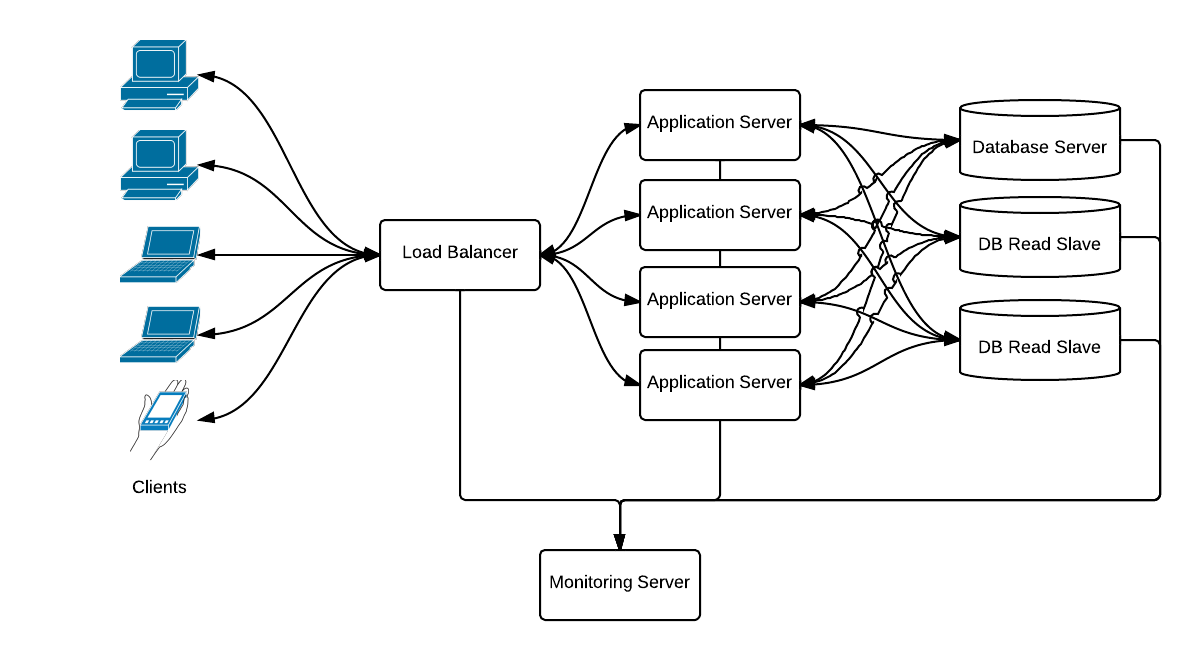
\includegraphics[width=\textwidth]{diagrams/highavailability.png}
\caption{Example architecture of a high availability application.}
\label{fig:highavailability}
\end{figure}

\section{High Availability Applications}
Not every system needs to be constantly scaled up and down. Applications that are not required to produce results in real-time can be scaled in order to produce a result in a specific amount of time. MapReduce \cite{dean2008mapreduce} systems are a prime example of this. Typically, the results produced by these systems are for analytical purposes and it is not expected for the results to be available immediately. Developers can set expectations for completion time and scale these systems accordingly. For example, our arts and crafts store produces a yearly report with detailed information about our worldwide sales. We could request this report at the end of the work day and scale our cluster such that a result will be ready by the next morning.

The services that would benefit most from a system which could automatically scale services are known as ``high availability'' applications. These are services which are often expected to produce results in less than a second and need to scale their computational resources based on demand in order to meet these performance goals. A few recognizable examples of high availability websites include Google \cite{google}, Facebook \cite{facebook}, Wikipedia \cite{wikipedia}, and Twitter \cite{twitter}. Each of these web sites must return information to the user in a reasonable amount of time or else the user will lose interest and leave. An example architecture of a high availability application can be seen in \Cref{fig:highavailability}. We see multiple application servers that host the application code sitting behind a load balancer. These application servers take requests from users, acquire the necessary data from the database, perform any required business logic, format a web page, and send the contend back to the user. All pieces of this system generate metrics which are then passed to the monitoring server. This data can then be used by operations engineers in order to make decisions about when to scale the different components of the system.

\section{Monitoring}
In order to meet the needs of high availability systems, it is important to collect as many metrics as possible to give insight into its performance. As one can see in \Cref{fig:highavailability}, every component of the system feeds data into the monitoring server. Just as with traditional capacity planning, monitoring tools are used to decide when it is time to scale.

\subsection{Measuring Throughput}
Of specific interest to this work is the measurement of application throughput. The throughput of a web application is defined as the number of requests a system can respond to within the span of a second. This metric is typically calculated using latency, the amount of time between when a request is made to a server and when it is responded to.

Services which offer service level agreements (SLAs) on latency measure their system throughput by finding the maximum number of requests per second a single node of the system can handle while still responding in less than the agreed upon time \cite{allspaw2010web}. Maintaining high throughput is important, so many providers, even if not bound by SLA, set standards for latency in order to optimize cost with customer satisfaction.

\section{Load Balancing}
If it is necessary for a horizontally scaled system to be public-facing then it is necessary for it to be load-balanced. Load balancers serve as gate keepers to distributed applications, routing requests to different servers to ensure an even distribution of load amongst them \cite{schlossnagle2006scalable}. You can see a load balancer between the clients and application servers in \Cref{fig:highavailability}. Load balancers can also serve other useful functions, such as geographically distributing load, checking the health of the hosts behind them to ensure requests aren't sent to failed hosts, and sending specific percentages of traffic to certain nodes for testing purposes. Metrics like latency and requests per second (the metrics necessary to calculate throughput) are most easily captured in the load balancer.

\section{Cloud Scaling Considerations}
\label{sec:considerations}
The cloud is a very different infrastructure than traditionally managed data centers. While the cloud provides many advantages, there are still important lessons to be learned from traditional scaling, as well as new challenges which must be taken under consideration when developing any scaling plan.

\paragraph{Hourly Billing.} Most cloud service providers charge based on an hourly cycle. This means that even if a node is only active for five minutes, it will be charged for a full hour of use. A good scaling plan should take this into account and should only shutdown nodes which are closest to a full hour of operation.

\paragraph{Acquisition Delay.} While the cloud has made the acquisition of computing power much faster than it has been in the past, it is still important to consider that nodes will take time to become operational. Not accounting for this delay can result in lost availability for a system and possible breach of SLAs. Scaling plans should consider this delay when requisitioning new nodes, it is important to make these requests properly in advance.

\paragraph{Diminishing Returns.} Adding one node to a single node cluster results in a roughly 100\% increase in resources; however, adding a single node to a cluster of thousands of nodes will have a much smaller effect. A good scaling plan ensures that a proper amount of resources is requested relative to the size of a system.

Cloud providers have no vested interest in services using only the optimal resources required to maintain availability. There is no motivation for them to help these services create effective scaling strategies which minimize wasteful use of compute time. The goal of this work is to fulfill this need and allow these systems to scale more effectively than ever before.

\section{Technologies Used}
The work presented in this paper leverages a few key technologies which we will introduce here and explain their relation to our systems.

\subsection{MapReduce}
MapReduce is a distributed computational framework for easily distributing the analysis of large data sets \cite{dean2008mapreduce}. It breaks distributed tasks down into two primary parts, the \texttt{map} and the \texttt{reduce} steps.The \texttt{map} step reads in one piece of input at a time (how this data is read is defined by the user) and then emits a series of key-value pairs which will then be sent to the \texttt{reduce}. The \texttt{reduce} is then run once per unique key emitted by the map and is passed the key along with all values which were emitted with that key in order to perform an aggregate calculation. A common example of a MapReduce application is counting the words in a book. The \texttt{map} takes in one line at a time and emits the number of occurences of every word on that line. The \texttt{reduce} then sums the counts for every word and the output is written to a file. A simple flow diagram explaining MapReduce can be seen in \Cref{fig:mapreduce}.

\begin{figure}
\centering
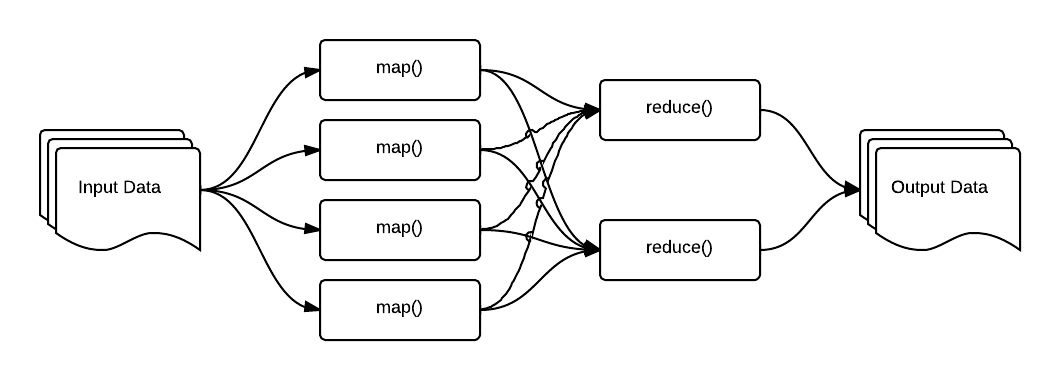
\includegraphics[width=\textwidth]{diagrams/mapreduce.png}
\caption{A simplified explanation of MapReduce}
\label{fig:mapreduce}
\end{figure}

In order to build the Wikipedia traffic data set, we processed a set of raw Wikipedia request logs using Hadoop \cite{hadoop} hosted on Amazon's Elastic Map Reduce \cite{emr} and wrote our job in Python using mrjob \cite{mrjob}, a library originally developed by Yelp for running Python code with Hadoop. For more information, see \Cref{ch:workloads}.

\subsection{CouchDB}
Much of the functionality of ARTS and CRAFTS is built on top of CouchDB \cite{couch}. CouchDB is a document store which allows for the storage of schema-less data in the format of JSON documents. At its core, CouchDB is a powerful key-value store. Storage of documents is primarily based on the specification of an \texttt{id} field which is used to retrieve the document later. CouchDB uses a REST API for all of its operations, so its complete functionality is accessible entirely though HTTP requests.

An important and powerful feature of CouchDB is incremental MapReduce. This functionality behaves in a fashion similar to what was described in the previous section. A user can specify a ``\texttt{view}'' which is a data transformation (\texttt{map}) and optional aggregation (\texttt{reduce}) selectively applied to documents in the database. These views are defined using Javascript or Coffeescript functions which every document is passed through upon insertion to the database as well as during subsequent updates. The results of the view are stored in a B+ tree which allows for quick retrieval of all documents emitted by the view, as well as ranges based on keys.

CouchDB also supports ``\texttt{list}'' functions. Also specified in Javascript, \texttt{list} functions are used to transform documents based up the method by which they are requested. For example, documents requested through a web browser can be transformed into an HTML document for more friendly viewing by end-users.

CRAFTS uses CouchDB as an intermediate store for metric data between itself and external monitoring services. CRAFTS leverages the incremental MapReduce feature to compute aggregates across this data as well. It also uses CouchDB to store intermediate data produced by the analysis pipeline. The web interface to CRAFTS uses \texttt{list} functions in order to transform the data into a format which can be used by the chart library used in the web interface. For more information, see \Cref{ch:datapipe}.
\chapter{Related Work}
\label{ch:related}
The scaling of hardware and software systems manifests itself in many different ways. Scaling can include operations such as purchasing of new hardware, the addition or reductions of resources available to a VM, or the addition or removal of VMs from a cluster. Since our work is primarily concerned with the automated scaling of virtual resources, the following sections focus on methods which have been presented in recent relevant literature.

\section{Reactive Scaling}
Reactive scaling is done in response to an increase in the load on a system. It requires little historical data and is typically done through threshold limits. A typical rule would be something of the form: ``if the average CPU utilization across all machines is greater than 75\% for more than 5 minutes, add another node to the cluster.'' This makes reactive scaling an invaluable tool for handling sudden load spikes. Conversely, reactive scaling can remove instances which have been idle for an extended period of time. Reactive scaling is offered by many cloud hosting providers including Amazon \cite{ec2autoscale} and Rackspace \cite{rackspace}. The problem with reactive scaling is that by the time the needed capacity comes online, it is possible that the load will have made a noticeable performance impact on the system, possibly breaking SLAs.

\section{Schedule-based Scaling}
In a schedule-based scaling environment, operations engineers define specific, possibly recurring, times when scaling events must occur. Schedules typically account for periodic traffic patterns and expected usage surges during holidays. This method, when used in conjunction with reactive scaling, can maintain availability during normal operation and handle unforeseen load without requiring constant observation by engineers. Schedule-based scaling is also a common offering among cloud providers \cite{ec2autoscale} \cite{rackspace}. However, schedule-based scaling is entirely static. Schedules must be manually defined by engineers and can often result in wasted capacity or losses in availability due to their static nature.

\section{Predictive Scaling}
Predictive scaling is a relatively new technique which seeks to solve the pitfalls of both reactive and schedule-based scaling. With predictive scaling, the system looks at historical usage patterns and attempts to predict future demand and to automatically scale accordingly. Predictive scaling is not a replacement for other techniques, but is a powerful addition to the scaling tool set. Reactive scaling can still handle unforeseen demand, and schedules can be used to handle events which may not be possible to derive from historical data. The following sections outline some commonly used algorithms found in recent predictive scaling literature.

\subsection{Fast Fourier Transform}
\label{sec:fft}
Fast Fourier transforms (FFTs) are used by Netflix's auto-scaling system, Scryer \cite{scryer}. It is also used in Google's PRESS system for scaling the size of VMs on a bare metal system \cite{gong2010press}. The fast Fourier transform is an algorithm which takes in a set of input points and converts them into the frequency domain. By removing frequencies which are not dominant and performing the inverse transformation, a smoother line which is still representative of the original data set can be extracted. This approach is able to handle prediction of periodic input data, as well as account for anomalous traffic like load spikes and averages.

An FFT algorithm is formally defined as any approach which can be used to calculate the result of a discrete Fourier transform (DFT) in $O(n log(n))$. The definition of the DFT can be found in \Cref{eq:dft}. The most commonly used FFT algorithm is the Cooley-Turkey FFT algorithm \cite{statistics}. This algorithm takes the DFT calculation for a sample size $N$ and breaks it up into smaller DFTs of size $N_1$ and $N_2$, taking a divide and conquer approach in order to achieve $O(n log(n))$.
\begin{equation}
\label{eq:dft}
X_k = \sum_{n=0}^{N-1} x_n e^{-i2\pi k \frac{n}{N}} \quad \forall k \in 0,\dots,N-1
\end{equation}

\subsection{Linear Regression}
\label{sec:regression}
As a supplement to FFTs, Scryer uses linear regression \cite{statistics} in its predictions \cite{scryer}. Linear regression takes a set of input points and attempts to produce the best-fit line through them. By selecting multiple points within a window of time on several different days, Scryer applies linear regression and can produce a prediction for demand during that window of time in the future. The problem with this approach is that it is very intolerant to spikes and outages. Removal of outliers can be used to mitigate this effect. Additionally, Scryer takes fewer samples within the window as it moves farther back in time in order to weigh recent data more heavily.

\subsubsection{Simple Linear Regression}
\label{sec:slr}
Since the nature of our temporal data is only two-dimensional (value over time) we can use a simple linear regression \cite{statistics}. A simple linear regression can be used to find the slope of the line, $\beta$, and the $y$-intercept, $\alpha$, as seen in \Cref{eq:line}.
%
\begin{equation}
\label{eq:line}
\begin{split}
y& = \alpha + \beta x \\
\beta& = \frac{\sum_{i=0}^{n}(x_i - \bar{x})(y_i - \bar{y})}{\sum_{i=0}^{n}(x_i - \bar{x})^2} \\
\alpha& = \bar{y} - \beta \bar{x} \\
\end{split}
\end{equation}

\subsubsection{Cook's Distance}
\label{sec:cook}
Although the Scryer paper does not outline the algorithm used for outlier detection, Cook's distance is an example of one such method. Cook's distance \cite{statistics} measures the influence that any given point has on the regression. By taking the Cook's distance of every point in the regression, we can filter the input data based on a configurable threshold so that outliers can be removed, then re-run our simple linear regression. Cook's distance for point $i$ is defined as follows:
%
\begin{equation}
\label{eq:cook}
D_i = \frac{\sum_{j=1}^{n}(\hat{y}_j - \hat{y}_{j(i)})^2}{p MSE}
\end{equation}
%
Where:
\begin{itemize}
\item $y_j$ is the predicted value given by the regression for point $j$.
\item $y_{j(i)}$ is the predicted value given by the regression where point $i$ has been excluded.
\item $p$ is the number of fitted parameters in the model. In our case, $p = 2$ (time and value).
\item $MSE$ is the average of the squares of the errors, or Mean Squared Error (MSE). This calculation can be seen in \Cref{eq:mse}.
\end{itemize}
%
\begin{equation}
\label{eq:mse}
MSE = \frac{1}{n} \sum_{i=0}^{n} (\hat{y}_i - y_i)^2
\end{equation}

\subsubsection{Theil-Sen Estimator}
\label{sec:tse}
We are using the Theil-Sen estimator for our own evaluation \cite{statistics}. The Theil-Sen estimator differs from a simple linear regression in that it is naturally insensitive to outliers. The Theil-Sen estimator of a set of points $(x_i,y_i)$ is defined as the median of all slopes $(y_j - y_i)/(x_j - x_i)$. The $y$-intercept can be calculated as the median of the values $y_i - mx_i$. The difference between a Theil-Sen estimator and a simple linear regression (outliers included) can be seen in \Cref{fig:regressioncmp}, where the solid line with the weakest slope is the result of a simple linear regression, the solid line with the greater slope represents the result of the Theil-Sen estimator, and the dashed line represents the ground truth which was used to generate the input samples.

\begin{figure}
\centering
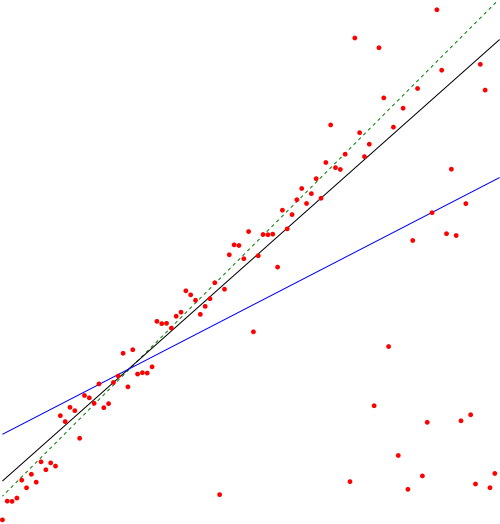
\includegraphics[width=200px]{diagrams/theilsen.png}
\caption{A comparison of the simple linear regression and Theil-Sen estimator methods.}
\label{fig:regressioncmp}
\end{figure}

\subsection{Discrete-time Markov Chain}
\label{sec:chains}
In Google's PRESS paper, the researchers used discrete-time Markov Chains \cite{statistics} to make short-term predictions when scaling VMs, specifically when no periodic trend can be detected in the input \cite{gong2010press}. A discrete-time Markov chain defines a set of states, and the probabilities of moving between them. PRESS divides resources into equal width value buckets and generates a probability matrix based on the probability of moving from one bin to another. This can be done by looking at historical data and observing past transitions. In order to calculate the probability distribution n samples in the future, PRESS used the Chapman-Kolmogorov equation \cite{statistics} seen in \Cref{eq:ckeq}. By taking the probability matrix and raising it to the $t$ power, where $t$ is the amount of time into the future which we would like to predict, we are given a new matrix which represents the probability of moving from any given state to another state $t$ time in the future.
\begin{equation}
\label{eq:ckeq}
P(t) = P^t
\end{equation}

\subsection{Exponential Smoothing}
The AppScale platform uses exponential smoothing in order to make short-term predictions on load \cite{bunch2012pluggable}. Exponential smoothing \cite{statistics} can also be referred to as exponential moving average. The smoothed value for any time $t$ is a weighted average between the previously observed value, $x_{t-1}$, and the previously smoothed value, $s_{t-1}$. The smoothing factor, $\alpha$, is a value between 0 and 1 which is used to compute the weighted average. A smaller $\alpha$ means more smoothing and a larger $\alpha$ means less smoothing.
\begin{equation}
\begin{split}
s_1& = x_0\\
s_t& = \alpha x_{t-1} + (1 - \alpha) s_{t-1}
\end{split}
\end{equation}

Normal exponential smoothing allows for predicting on observation into the future. For our purposes, this is not enough. A single observation into the future is unlikely to account for VM acquisition delay, we require a more powerful forecasting method. A technique called ``double exponential smoothing'' \cite{statistics} allows for predictions further into the future by adding a second smoothing factor, $\beta$, which is intended to account for trends in the previously observed data. The equation for double exponential smoothing is as follows:
\begin{equation}
\begin{split}
s_1& = x_1\\
b_1& = x_1 - x_0\\
s_{t}& = \alpha x_{t} + (1-\alpha)(s_{t-1} + b_{t-1})\\
b_{t}& = \beta (s_t - s_{t-1}) + (1-\beta)b_{t-1}\\
\end{split}
\end{equation}
The principles regarding how $\beta$ smooths are the same as $\alpha$. In order to predict values in the future, the following equation can be used:
\begin{equation}
F_{t+m} = s_t + mb_t
\end{equation}
Where $m$ is the number of observations into the future for which the prediction is being made.

%\section{Related Systems}
%While they have been referenced in previous section, this section will explore the different existing predictive scaling systems in current literature.

%\subsection{PRESS}
%PRESS is a system developed at Google for scaling VM resources on a bare-metal machine. Unlike CRAFTS, PRESS' goal is vertical scaling

%\subsection{Scryer}

%\subsection{AppScale}

\section{Workload Simulation}
Most web workload simulation tools try to simulate a realistic distribution of operations in order to evaluate the performance of a cluster. Most of these workloads do not take into account the time-series usage patterns which are the focus of our research, but some of the concepts used were an important inspiration in building our own tool.

\subsection{Rain}
The Rain \cite{beitch2010rain} workload generator is a toolkit designed to create realistic workloads for cloud applications. Users build ``generators'' which define a set of actions which a user on the site may take and a probability matrix based on the probability of one of those actions occurring after another. Using Markov chains, Rain simulates the sessions of a specified number of users over time. Workload specifications can fluctuate the number of concurrent users at any given time, but this data cannot be dynamically generated by Rain.

\subsection{Xerxes}
Xerxes is a resource-load generation tool for job-based workloads \cite{kesavan2012xerxes}. It is designed to stress-test large distributed systems by creating actual resource utilization on worker nodes. The Xerxes architecture contains a master node which will generate workloads for the slave nodes to execute based on either an existing resource utilization trace or a specified statistical distribution. Statistical workload specifications can be of either a gaussian or uniform distribution and may also include utilization spikes of pre-configured durations and magnitudes.

\subsection{WikiBench}
The WikiBench tool most closely aligns with the goals of our own research. WikiBench ``allows one to stress-test systems designed to host Web applications (application servers, load balancers, databases, Cloud computing platforms, etc.). \cite{wikibench}'' By using a real set of traces recorded from Wikipedia in 2007, WikiBench provides the tools to replay these traces against a working MediaWiki installation. For the purposes of our work, the most interesting part of WikiBench is the Wikipedia traces which come with it, two months of real request logs spanning September and October of 2007. A time-series plot of this data can be seen in \Cref{fig:wikibench}.

\begin{figure}
\centering
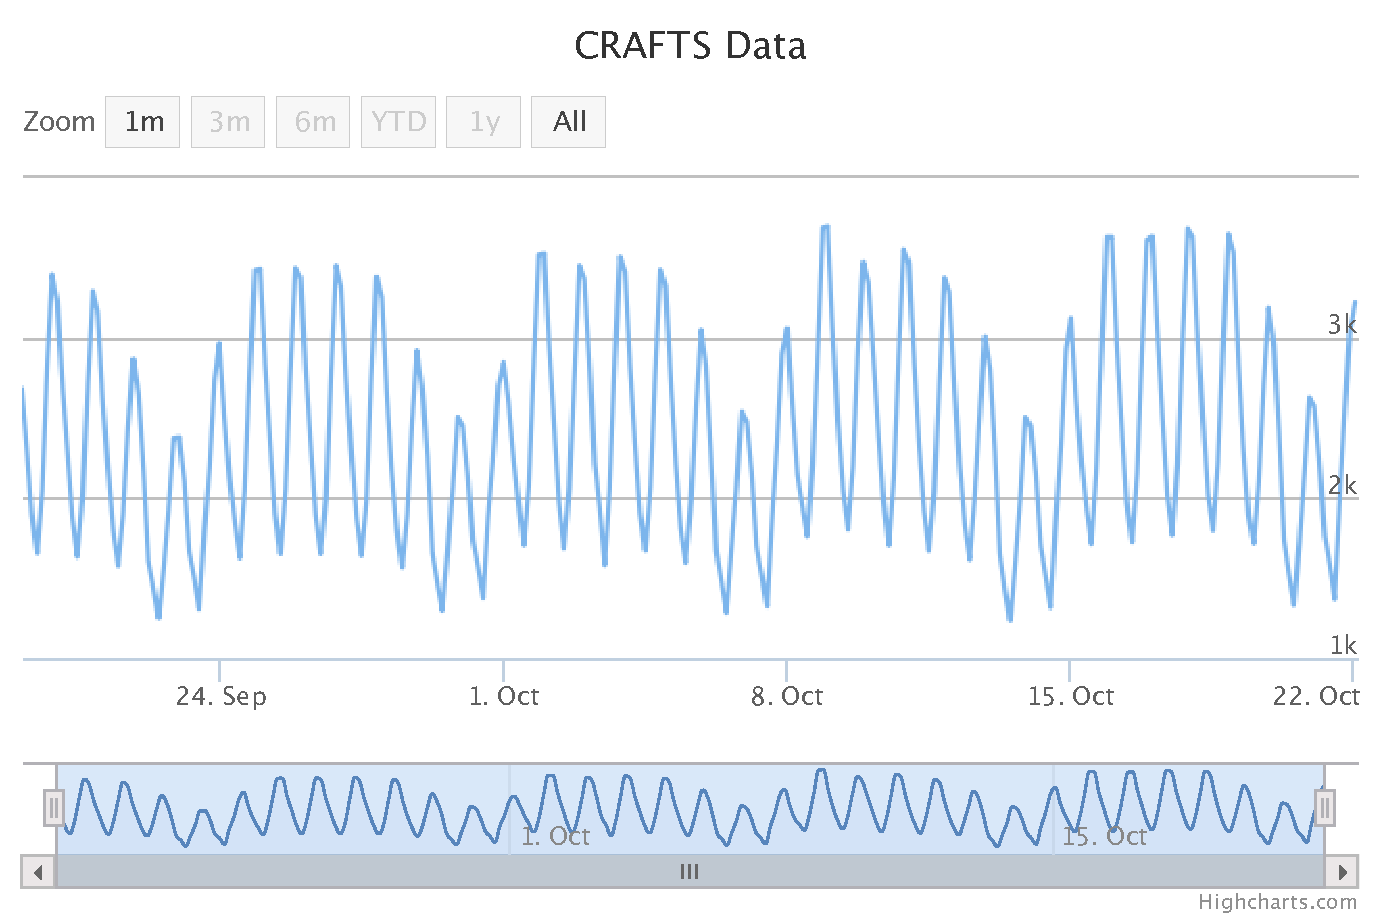
\includegraphics[width=\textwidth]{charts/wikibench.pdf}
\caption{A time-series plot of Wikipedia input data.}
\label{fig:wikibench}
\end{figure}

\subsection{Older Datasets}
While there are few recent request trace workloads available to researchers, there are a few historical datasets which can still be applied to modern research. These datasets have a significantly lower magnitude, but our primary concern is the trends present in the data which can be measured regardless of magnitude. Google's PRESS paper used two historical datasets in their own benchmarks, ClarkNet and the FIFA '98 website \cite{gong2010press}.

\paragraph{ClarkNet.} The ClarkNet dataset is comprised of two weeks of traffic through the Metro Baltimore Washington DC area ISP ClarkNet. The datset spans from August 28, 1995 to September 10, 1995 and contains a total of 3.3 million requests \cite{clarknet}. A time-series plot of this data can be seen in \Cref{fig:clarknet}.

\begin{figure}
\centering
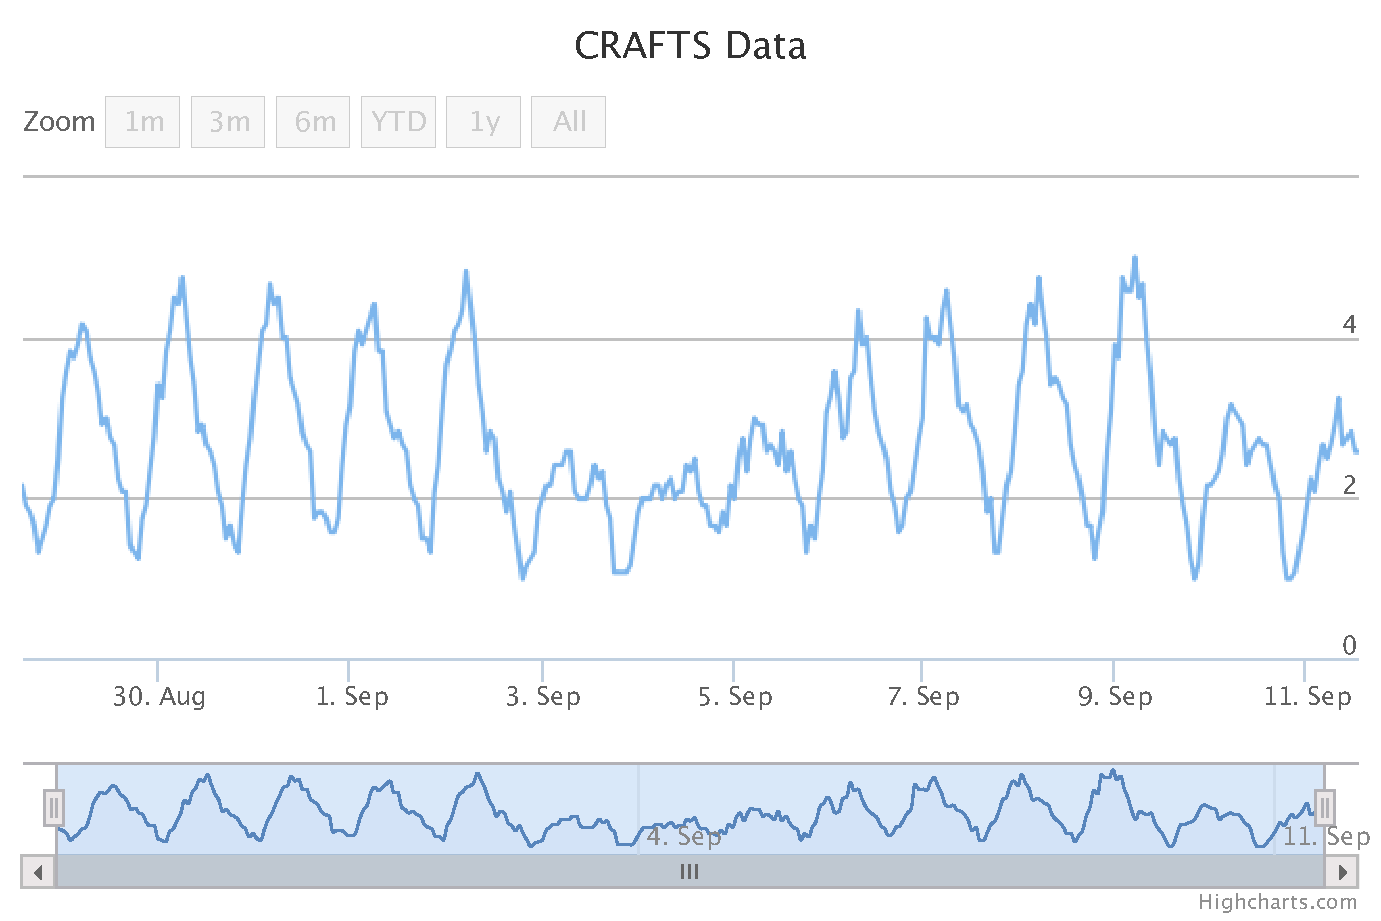
\includegraphics[width=\textwidth]{charts/clarknet.pdf}
\caption{A time-series plot of ClarkNet input data.}
\label{fig:clarknet}
\end{figure}

\paragraph{FIFA '98.} The 1998 FIFA World Cup took place in Paris, France from June 10th to July 12th. The FIFA '98 dataset is comprised of server request logs to the world cup website between April 30th and July 26th. A total of 1.3 billion requests were made during this period. This dataset is especially interesting because it contains not only the expected diurnal traffic patterns, but a large peak during the cup itself. This kind of dataset would likely throw off predictive mechanisms which rely solely on periodicity \cite{worldcup}. A time-series plot of this data can be seen in \Cref{fig:worldcup}.

\begin{figure}
\centering
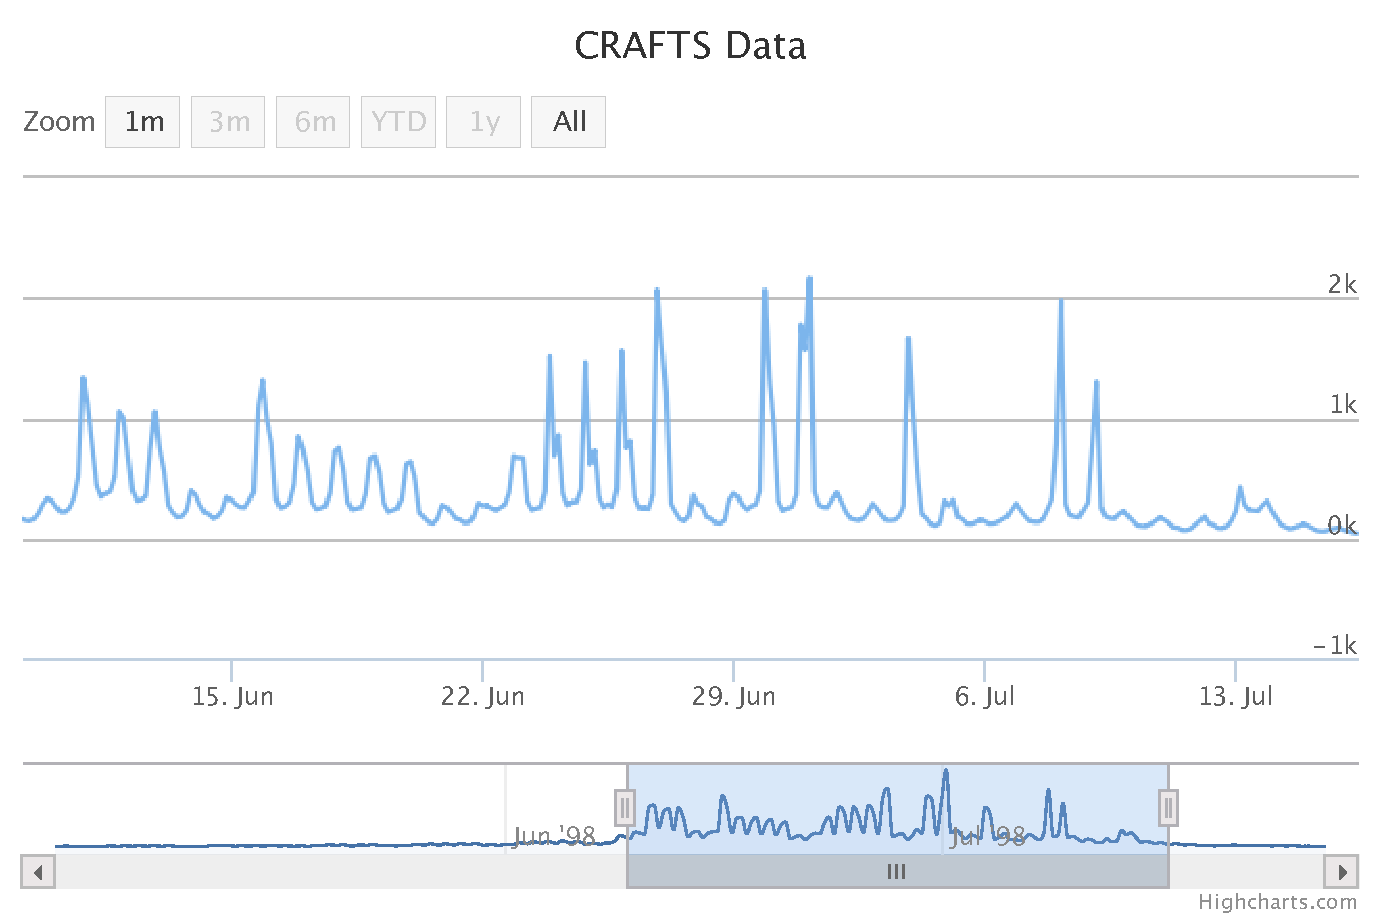
\includegraphics[width=\textwidth]{charts/worldcup.pdf}
\caption{A time-series plot of the 1998 Worldcup input data.}
\label{fig:worldcup}
\end{figure}

\chapter{System Overview}
\label{ch:overview}
CRAFTS (Cloud Resource Anticipation For Timing Scaling) is a system for automatically identifying application throughput and predictively scaling cloud computing resources based on historical data. By taking past monitoring data such as requests per second and request latency, CRAFTS calculates the optimal throughput of the application it is monitoring and uses this data to make a direct translation between incoming traffic and the number of servers required to handle the capacity and maintain availability.

Since it is uncommon for companies to publish exact numbers about their web traffic over large periods of time, evaluating the effectiveness of CRAFTS' prediction algorithms in a real world scenario is difficult to accomplish. To fill this need, we have developed ARTS (Automated Request Trace Simulator), a request based workload generation tool for constructing diverse and realistic request patterns for modern web applications. ARTS allows us to evaluate CRAFTS' algorithms on a wide range of scenarios.

\section{Requirements}
When deployed, CRAFTS would serve a mission-critical function to the service which it monitors. Because of this, it is important that CRAFTS meet a very strict set of requirements to ensure that engineers can be confident in its predictions.

\subsection{CRAFTS Requirements}

\paragraph{Modular.} There is no ``one size fits all'' way to manage a cluster. It is important that the different pieces of CRAFTS can act independently of one another so alternate modules can be swapped in based on the application's needs. Modularity allows CRAFTS to integrate with many different monitoring systems and cloud service providers. This also means that CRAFTS can swap in different prediction methods based on what method would work best for the traffic patterns seen by the application which it is monitoring.

\paragraph{Available.} Because CRAFTS is responsible for the availability of entire systems, many of which may offer their own service level agreements on performance and availability, CRAFTS shall support some method of crash recovery which will allow it to continue to make predictions even in the event of a failure.

\paragraph{Independent.} CRAFTS must not require knowledge of application code in order to make its predictions. While this information can be provided to and used by CRAFTS, it should only serve to increase the accuracy of CRAFTS predictions. All of CRAFTS predictions should be made solely based on metrics available through the monitoring API which it has access to.

\paragraph{Scalable.} The services which CRAFTS monitors will likely not be comprised of a single component type. For example, many web sites have front-end servers which handle the rendering of HTML templates to be returned to the browser, as well as application servers which handle the business logic of the application. CRAFTS must provide a mechanism to scale multiple components independently of one another.

\paragraph{Configurable.} CRAFTS will be using throughput to calculate how many nodes are required to handle load, but requirements for latency vary wildly from application to application, it is necessary for CRAFTS to allow for the specification of desired latency in order to make cost-effective scaling decisions.

\paragraph{Anomalous Load Tolerance.} CRAFTS predictions need to tolerate the presence of anomalies in monitoring data. This includes system outages, usage spikes from denial of service attacks, and viral traffic. While it is necessary to account for this data in real-time scaling decisions, it has a negative impact on the quality of historical data used for making predictions.

\paragraph{Self-tuning.} If the throughput of a system component fluctuates, CRAFTS shall take this information into account in its predictions. Additionally, if CRAFTS detects that it is consistently over or under allocating capacity, it must take steps to alter future predictions to better fit actual demand.

\paragraph{User Interface.} It should be as simple as possible for engineers to get insight into the effectiveness of CRAFTS' predictions. The most straightforward way to accomplish this is to offer a simple user interface which can chart CRAFTS predicted demand vs. observed demand.

\subsection{ARTS Requirements}

\paragraph{Reproducible.} In order to perform effective benchmarking of CRAFTS' prediction techniques, workloads produced by ARTS need to reproducible. This way, prediction methods can be re-tuned and tested against the same set of test data and allow for a direct comparison of results.

\paragraph{Realistic.} Usage patterns produced by ARTS shall be as representative of real-world situations as possible. Request-based traffic cannot be realistically modeled with a continuous curve, minor and even major fluctuations in traffic around a central curve are inevitable. Patterns also exist over periods larger than a single day. For example, most applications not only experience traffic periodicity on a daily basis, but also show patterns in weekly access. Hopefully, these applications are also seeing growth over time as well. Being able to handle astronomic rises to popularity is a staple of the cloud and shall be represented in the workloads used to test CRAFTS.

\paragraph{Comprehensive.} ARTS shall be able to test every requirement of CRAFTS. For example, ARTS must be able to produce workloads which show small changes over time or changes in underlying application performance which would force CRAFTS to automatically tune its algorithms. These workloads must also include anomalous activity like outages and usage spikes to ensure CRAFTS can account for them.

% CRAFTS
\chapter{CRAFTS Data Pipeline}
\label{ch:datapipe}
The goal of the CRAFTS data pipeline design is to be as modular as possible. We take a page from the Unix philosophy, every component of CRAFTS is designed to do one thing, do it well, and be easily swappable with alternate modules. A graphical representation of the CRAFTS data pipeline can be seen in \Cref{fig:workflow}.

\begin{figure}
    \centering
      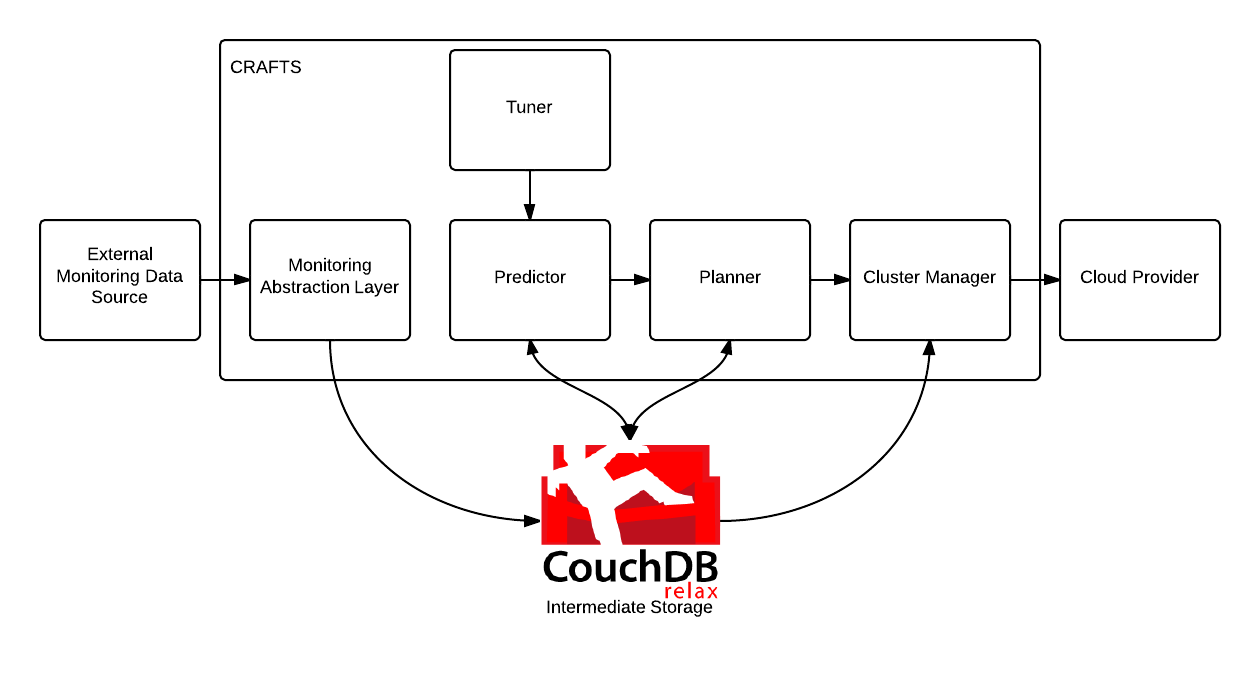
\includegraphics[width=\textwidth]{diagrams/datapipeline.png}
      \caption{Flowchart describing the CRAFTS workflow.}
      \label{fig:workflow}
\end{figure}

Data which is used for predictions is first passed in through the Monitor Abstraction Layer (\textsf{MAL}). Here, the data is put into intermediate storage for redundancy and so that aggregate calculations can be made through CouchDB's incremental MapReduce views. This data is then used by the \textsf{predictor} in order to predict future demand for the resource. These results are then also saved back to intermediate storage. Prediction data is then read by the \textsf{planner} which translates this data to a number of nodes required to maintain availability. The plan generated by the \textsf{planner} is then carried out by the \textsf{cluster manager} which makes the appropriate external API calls to acquire the cloud resources. CRAFTS also constantly tests its prediction algorithms on observed historical data and tunes prediction parameters in order to ensure the most accurate predictions possible. The rest of this chapter describes each of the data pipeline components in much greater detail.

\section{Monitor Abstraction Layer}
Data first enters the CRAFTS pipeline through the Monitoring Abstraction Layer (\textsf{MAL}). Since CRAFTS does not implement its own monitoring, the \textsf{MAL} is designed to provide a common API that allows CRAFTS to query external monitoring sources for cluster performance information. In order to mitigate load on the monitoring service, the \textsf{MAL} sends bulk requests for data at a configurable interval. This interval is called the \textbf{monitoring interval}. The data is then stored in an intermediary CouchDB database which can then be queried by CRAFTS' other components.

\section{Intermediate Storage}
Here, we describe how CRAFTS represents the monitoring data placed into intermediate storage by the \textsf{\textsf{MAL}}. This data is both inserted and stored as JSON. A diagram describing the different entities and attributes stored can be seen in \Cref{fig:datamodel}. Since CRAFTS can be implemented as a multi-tenant system, the highest level entity is that of the \textbf{tenant}. A tenant represents a single ``customer'' of CRAFTS. Data between tenants is isolated and configured independently. Tenants are implemented as CouchDB users who are given permissions to access the CRAFTS database as well as custom permissions which specify the roles they control. \textbf{Roles} are independent components of a system which are scaled independently. The primary data used by CRAFTS are samples. \textbf{Samples} are metrics collected at a given point in time. A sample document holds metrics for all the hosts assigned to the parent role at that timestamp, examples can be seen in \Cref{ap:storage}. Using CouchDB's incremental MapReduce, the sample also contains aggregates for each metric among all the hosts. These aggregates include max, min, average, count, sum, and variance. This aggregate data serves as the primary input for the \textsf{predictor}.

\begin{figure}
\centering
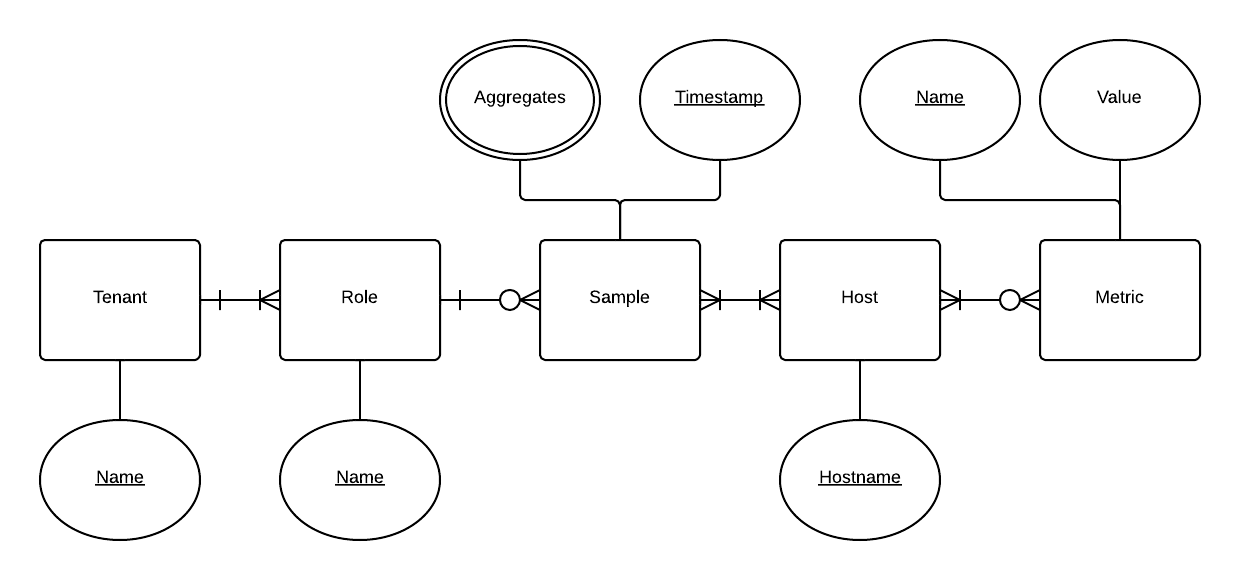
\includegraphics[width=\textwidth]{diagrams/datamodel.png}
\caption{An ER diagram describing how CRAFTS represents monitoring data.}
\label{fig:datamodel}
\end{figure}

\section{Predictor}
The purpose of the \textsf{predictor} is to determine the demand for a specific resource over the next \textbf{prediction horizon}. A prediction horizon is defined as how far into the future CRAFTS will attempt to make predictions. While which metric is predicted by the \textsf{predictor} is configurable, it typically is requests per second. Requests per second is an ideal metric because it is independent of the performance of the cluster (Netflix engineers made the same observation when building Scryer \cite{scryer}). Other useful values could include total database queries or cache requests. The \textsf{predictor} has no knowledge of the current state of the cluster, its job is solely to predict demand. The predictions generated by the \textsf{predictor} are based on a training set called the \textbf{training window}. The training window is a configurable length of time that the \textsf{predictor} may use in order to make its predictions. Details of the different prediction algorithms can be found in \Cref{ch:policies}.

Predictors may also specify configurable parameters which can be manipulated by the \textsf{tuner} in order to ensure the most accurate predictions possible. Examples of such parameters could include threshold values or offsets.

Like the \textsf{MAL}, predictors run at an interval, this interval is called the \textbf{prediction interval}. Keep in mind that the scaling interval and prediction interval are different values. A prediction interval should never be longer than the length of a prediction horizon, as this would cause there to be a period of time for which no prediction has been made. The predicted demand for the next prediction horizon is then passed to the \textsf{planner}.

\section{Planner}
The \textsf{planner} takes in the projected resource demand from the \textsf{predictor} and generates a scaling plan which is stored in the intermediate store and carried out by the \nameref{sec:clustermanager}. Generating a scaling plan involves a number of considerations that are outlined below.

\subsection{Throughput}
In order to make a translation between the predicted resource utilization and the number of nodes required to handle the demand, it is necessary for the \textsf{planner} to know the throughput of the system. To do this, the \textsf{planner} uses request and latency information acquired from the \textsf{MAL} to calculate throughput. For our purposes, we define throughput as
\begin{quote}
the maximum number of requests per second which can be served while latency is kept under a configurable value.
\end{quote}
Throughput can also be overridden manually if desired.

\subsection{VM Acquisition Time}
Since VMs will not become available the moment they are requested, it is important that the \textsf{planner} requests new nodes far enough in advance that they are operational by the time they are needed. Since this value is difficult to determine automatically, CRAFTS uses a default value of 15 minutes, but this can be overridden by the user.

\subsection{Manual Overrides}
Sometimes it is necessary to account for events which are difficult to predict. For example, holiday traffic can cause massive spikes in load, but only for a single day out of the year. This makes it difficult for CRAFTS to predict these kinds of events. Because of this, the \textsf{planner} can be overridden and a number of nodes can be specified manually to ensure that these events are handled properly, without loss to availability.

\subsection{Linear Transformation}
The \textsf{planner} assumes that the \textsf{predictor's} output is correct and makes no attempt to detect possible anomalies in the data. It does, however, add a configurable linear transformation to the prediction data. This is not done to counteract any possible error on the \textsf{predictor's} part, but instead to provide a small amount of buffer capacity in case of an anomalous spike.

\section{Cluster Manager}
\label{sec:clustermanager}
It is the \textsf{cluster manager}'s responsibility to act as a liaison between the \textsf{planner} and the cloud service which hosts the application. The \textsf{planner} will make direct calls to the \textsf{cluster manager} to schedule scaling events at certain times. The \textsf{cluster manager} must then make the appropriate calls to the host service in order to ensure that the specified number of nodes are launched at the specified time. CRAFTS also supplies a ``null'' cluster manager which will carry out no scaling actions. This can be useful when simply evaluating CRAFTS prediction methods.

\section{Tuner}
\label{sec:tuner}
It is difficult, if not impossible to assert that one prediction algorithm with one set of parameters will guarantee optimal predictions for every type of workload. For this reason, CRAFTS allows prediction algorithms to specify a set of parameters which may be tuned in order to optimize prediction accuracy. The tuner applies brute-force optimization to the \textsf{predictor}'s parameters and uses the average of the root-mean square deviation on a temporal validation as the objective function. The following sections break down and define the equations used by the tuner.

\subsection{Brute-force Optimization}
Since the predictors which we have implemented in this work have very few parameters (at most two) we have chosen to simply brute-force the parameter space rather than opting for a more elegant solution. Brute-force optimization navigates the parameter space within set bounds and samples at specified intervals. If prediction methods implemented in the future require more advanced optimizations methods, a new module can be easily swapped in.

\subsection{Temporal Validation}
Temporal validation is a technique in which a data set is partitioned into subsets where analysis is performed on one subset, the training set, and then applied to the other subset, the validation set. For the purposes of our tuning analysis, we run temporal validation using a shifting window. This window begins at the start of our known dataset, runs predictions for the next prediction horizon and then shifts forward by some interval. The resulting prediction horizons are then evaluated against the observed data using the methods outlined in the following section.

\subsection{Average of Root-mean-square Deviation}
The resulting prediction horizons are compared to the observed data using Root-mean-square deviation (RMSD). RMSD is an error measurement which takes the square root of the sum of the squared difference between the predicted and observed value divided by the sample size. The equation for RMSD can be seen in \Cref{eq:rmsd}. The RMSD is then taken for every prediction horizon. The resulting value forms the output of the objective function used in our optimization.

\begin{equation}
\label{eq:rmsd}
RSMD = \sqrt{\frac{\sum_{t=1}^n (\hat{y}_t - y_t) ^ 2}{n}}
\end{equation}
\chapter{CRAFTS Architecture}
\label{ch:architecture}
CRAFTS is built to be as simple to deploy and configure as possible. The \texttt{crafts-cli} script provides options for setting up a CRAFTS database within CouchDB, as well as automatically loading all of the view and list functions CRAFTS requires to operate.

Once the database is configured, the CRAFTS daemon, \texttt{craftsd}, can be launched. \texttt{craftsd} is the primary executable for running the CRAFTS service. It takes in the CouchDB URL, name of the database, and the configuration document ID as parameters. The rest of this chapter goes into detail about how CRAFTS can be deployed, how it handles errors, how it can be configured, and how to access its data through the web UI.

\section{Deployment}
In order to make CRAFTS as accommodating of different system configurations and workflows as possible, it supports a number of methods of deployment. Detailed instructions for each method can be found in \Cref{ap:installing}

\subsection{Building from Source}
CRAFTS uses a Python utility called VirtualEnv which packages all of its dependencies, including a Python binary, together with the source code. Running CRAFTS from source is as easy as downloading or cloning the source repository, configuring the database using \texttt{crafts-cli}, and launching the CRAFTS daemon, \texttt{craftsd}.

\subsection{Installing with Pip}
CRAFTS is registered with the Python Package Index (PyPI) and can be installed on any machine running Python 2.7 using \texttt{pip}. Pip is the recommended Python packaging manager and can be used to install packages, their dependencies, as well as set up services.

\subsection{Docker}
Docker is a wrapper around Linux containers, an OS-level virtualization solution for running isolated Linux systems on a single host. Docker is rapidly growing in popularity as a deployment tool due to its ease of use and ability to run on almost any modern Linux based system without the performance overhead of traditional virtual machines.

CRAFTS can be built as a complete docker container. This container includes a pre-configured CouchDB instance and only requires the specification of a configuration file to be loaded into Couch on startup.

\subsection{Vagrant}
Vagrant is a headless virtual machine manager which allows for easy creation and management of development environments. CRAFTS supplies a Vagrantfile for easy creation of a development environment which includes the CRAFTS source code and all necessary dependencies, including a running CouchDB instance.

\section{Command-line Setup Utility}
CRAFTS offers a command-line setup utility called \texttt{crafts-cli}. The utility provides three commands: \texttt{init}, \texttt{update}, and \texttt{clear}. The \texttt{init} command takes CouchDB connection information and a configuration file as parameters and creates a database for CRAFTS in CouchDB. It also automatically creates all of the view and list functions necessary for CRAFTS to run and upload the specified configuration document. Mostly for debugging purposes, the \texttt{update} command re-uploads all of the view and list functions to CouchDB. Finally, the \texttt{clear} command can be used to remove the CRAFTS database from CouchDB.

\section{Configuring CRAFTS}
All of CRAFTS' configuration is pulled from the document specified when \texttt{craftsd} is launched. This means that there can be more than one configuration stored in the database, but one must be chosen at startup. All instances of \texttt{craftsd} should use the same configuration in order to avoid undefined behavior. The following sections discuss some of the more important aspects of configuration. A more detailed explanation of the CRAFTS configuration format and its paramaters can be found in \Cref{ap:craftsconfig}.

\subsection{Choosing Modules}
When \texttt{craftsd} downloads the configuration, it dynamically imports the modules specified in their respective fields. If a module requires its own additional configuration, this information can be stored under a key of the same name in the configuration. This is not a required naming convention because the entire configuration is passed to all modules, but it is a good practice to avoid confusion.

\subsection{Logging}
\texttt{craftsd} supports Python logging configuration files as attachments to the configuration document which will then be read on startup. CRAFTS also offers a special handler for putting log information back into CouchDB called Glitter. Glitter takes Python LogRecord objects and puts all of their attributes into a JSON document for storage in CouchDB. This makes the logs queryable through CouchDB views and easy to monitor remotely. This is especially useful in the event of a fail-over, all \texttt{craftsd} logging data stays contained in CRAFTS' main dependency.

\section{CRAFTS Web UI}
CRAFTS provides a web interface which displays its predictions and scaling plans laid over observed load. This allows engineers a visual method of validating the accuracy of CRAFTS decisions. This interface also includes markers for events such as when a tuning was run, as well as the results of that tuning. The web server is built in Python using the Flask framework and the charts are built using the Highcharts Highstocks Javascript library.

The web server serves as a proxy between the user interface and CouchDB. The server will ensure that the logged-in user has permissions required to view the requested data and to make queries to CouchDB list functions to retrieve the displayed data.

\begin{figure}
\centering
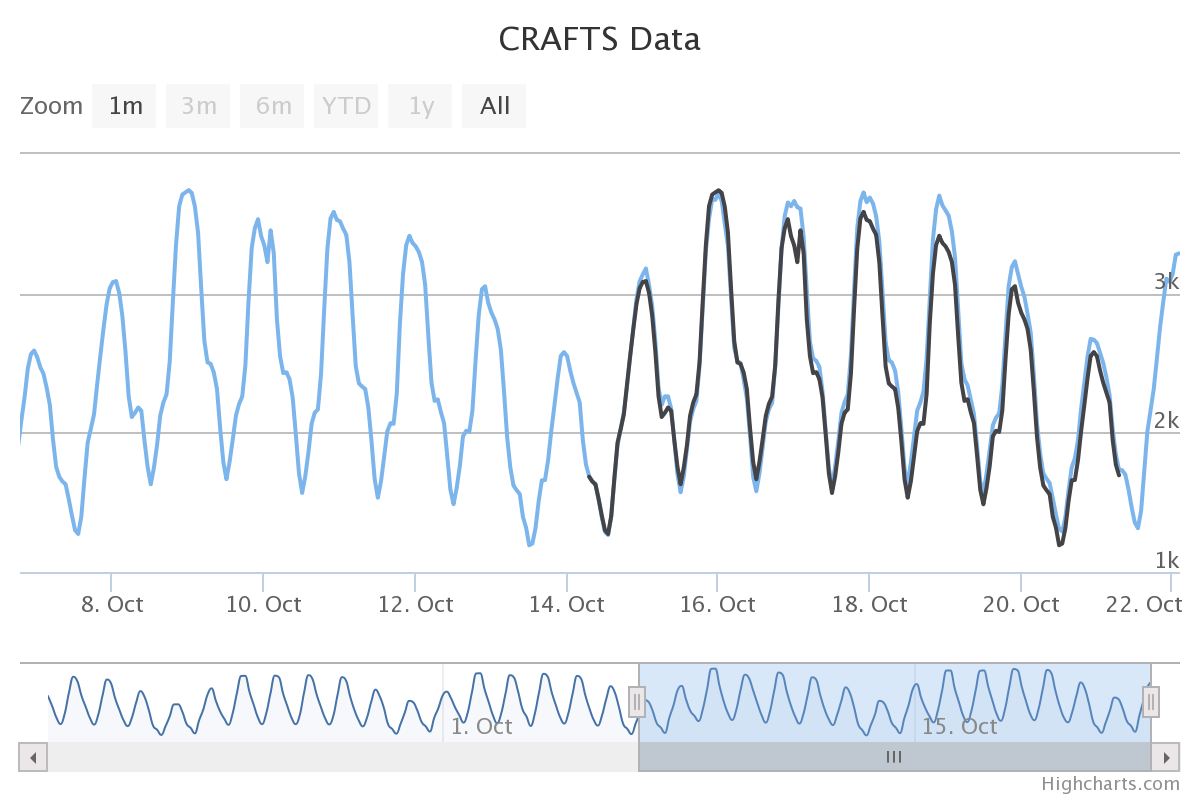
\includegraphics[width=\textwidth]{diagrams/webui.png}
\caption{The CRAFTS web interface}
\label{fig:webui}
\end{figure}

% ARTS
\chapter{ARTS Design}
\label{ch:arts}

\section{Layered Design}
ARTS uses continuous transformations as well as discrete-time events in order to generate realistic workloads. To make these workloads more complex, ARTS may use multiple transformations and apply them on top of each other. The following sections define the different types of transformations and events supported by ARTS as well as how they interact.

\subsection{Workload Base}
The base serves to give the other transformations a set of initial values to perform transformations on. ARTS supports two kinds of bases, file and value. The file base reads in a newline delimited file of unix timestamp and value pairs. The value base takes a baseline value and duration as parameters and applies the baseline value constantly for the entire duration of the workload.

\subsection{Continuous Transformations}
Continuous transformations are functions which will be applied to the entire generated dataset. Multiple continuous transformations can be layered on top of each other in order to obtain more diverse data sets. These layers can be configured to either be summed with the current workload or be applied as a multiplier.

\paragraph{Sinusoid.} Sinusoids are used to represent normal patterns seen in traffic. The resulting sine wave is centered around positive one and applied as a multiplier to the existing workload. The sinusoid transform takes an amplitude between zero and one and a frequency specified in days as parameters.

\paragraph{Linear.} In order to represent steady growth (or decay) seen in the real-world traffic, we offer a linear transformation. The linear transformation takes a slope as a parameter and applies that slope to each point in the workload.

\paragraph{Blur.} Real world traffic doesn't behave like a nice straight line, there are constant minor fluctuations in traffic patterns. The blur transformation takes the current workload and adds noise based on the Gaussian distribution. Using the current data point as the mean and a configurable standard deviation, a new value is generated and inserted back into the workload.

\subsection{Discrete-time Events}
A discrete-time event represents an anomaly in the input data which can be difficult to predict and could invalidate historical data. These events can occur multiple times and are configured with start and end times within the workload. ARTS supports the following discrete-time events:
\begin{itemize}
    \item Outages, a period of time in which all generated data is zero.
    \item Usage spikes, a short period of time when a large multiplier is applied to the base load.
\end{itemize}

\section{Output}
Workloads output by ARTS are passed to handlers. Handlers are called as each value is generated for processing. For our purposes, we have built a handler which inserts each data point into the CRAFTS intermediate store. We also provide a file handler so that workloads may be output to file and run again in the future.

\section{Reading from File}
ARTS can read data from an input file and either directly pass the values to handlers or use the data as a basis for a new workload, applying continuous transformations and discrete-time events on top of it. This can be useful if we want to apply discrete-time events to real-world data sets to see how it might change the accuracy of our predictions.

\section{Job Configuration}
ARTS takes a JSON configuration file as input. This file specifies the different layers and events, as well as their parameters, which the job will be comprised of. The format of this file can be found in \Cref{ap:artsconfig}.

% Evaluation
\chapter{Predictors}
\label{ch:policies}
CRAFTS is designed to be able to apply a series of different prediction algorithms. This chapter outlines the predictors we have implemented and intend to evaluate.

\section{Translation}
As a baseline, CRAFTS takes the data from the previous training window and translates it onto the next scaling cycle. In the context of the Wikipedia workload, the translation predictor takes the previous week's traffic and overlays it onto the next week. Since it assumes the next week's traffic will be identical to the previous week, the translation predictor is intolerant to both usage spikes and outages. The translation predictor has no parameters which are configurable by the \textsf{tuner}.

\section{Fast Fourier Transform}
The fast Fourier transform predictor applies the fast Fourier transform algorithm specified in \Cref{sec:fft} to all of the values in the training window and then filters out the least prominent frequencies. What percentage of frequencies are removed is a parameter configurable by the \textsf{tuner}. An inverse fast Fourier transform is then performed on the data to convert it back from the frequency domain to the time domain. The result is then used as the prediction for the next prediction horizon. 

By filtering out the least prominent frequencies, the FFT predictor is resistant to both outages and usage spikes. This is because these events should be sparse and non-repeating, or else they would be part of normal traffic patterns. Since these events are isolated, their frequencies will not be prominent in the frequency domain produced by the FFT and are likely to be filtered out.

\begin{algorithm}[H]
\KwData{$W =$ Training window data}
\KwResult{$P =$ Prediction horizon data}
\Begin{
    $freqDom = FFT(W)$\;
    $threshold = sort(freqDom)[len(freqDom) / 2]$\;
    \For{$freq \in freqDom$}{
        \If{$freq < threshold$}{
            $freq = 0$\;
        }
    }
    $P = inverseFFT(freqDom)$\;
}
\caption{FFT predictor}
\end{algorithm}

\section{Linear Regression}
The linear regression predictor applies linear regression on data points from previous days at similar times in the training window in order to predict what traffic will look like on future days at that time. For each time in the prediction horizon the linear regression predictor looks back at that time in all previous days in the training window, samples a set of points around that time, and applies linear regression. The number of points sampled around each time is configured by the \textsf{tuner}.

\begin{algorithm}[H]
\KwData{$W =$ Training window data \\
        $start =$ Time of the first prediction \\
        $interval =$ Time between each observation \\
        $end =$ Time of the last prediction}
\KwResult{$P =$ Prediction horizon data}
\Begin{
    \For{$pTime = start; pTime < end; time += interval$}{
        $rWindow =$ The points surrounding $pTime$ from the previous weeks in $W$\;
        
        $slopes = []$\;
        \For{$(valueA, timeA) \in rWindow$}{
            \For{$(valueB, timeB) \in rWindow$}{
                $slopes.append((valueB - valueA) / (timeB - timeA))$\;
            }
        }
        
        $slope = sort(slopes)[len(slopes) / 2]$\;
        
        $lines = []$\;
        \For{$(value, time) \in rWindow$}{
            $lines.append(value - time * slope)$\;
        }
        
        $intercept = sort(lines)[len(lines) / 2]$\;
        
        $P.append(pTime * slope + intercept)$\;
    }
}
\caption{Regression Predictor}
\end{algorithm}

\section{Discrete-time Markov Chain}
In order to make predictions using discrete-time Markov chains, \Cref{sec:chains}, this predictor uses all of the data in the training window in order to build the probability matrix. The number of buckets in the probability matrix is configured by the \textsf{tuner}. A data point $t$ time in the future is then estimated. The value of $t$ is configurable, but can never be smaller than the amount of time it takes to launch a VM. This is because predictions must be made far enough into the future that any necessary nodes can be brought online in time to handle the load at the time predicted.

\begin{algorithm}[H]
\KwData{$W =$ Training window data \\
        $t =$ Number of observations into the future to be predicted}
\KwResult{$P =$ Prediction horizon data}
\Begin{
    $pMatrix = [NUM\_BUCKETS][NUM\_BUCKETS]$\;
    \For{$i = 0; i < len(W) - 1; i++$}{
        $startBucket = bucket(W[i])$\;
        $endBucket = bucket(W[i + 1])$\;
        $pMatrix[startBucket][endBucket] += 1$\;
    }
    
    \For{$elem \in pMatrix$}{
        $elem = elem / len(W)$\;
    }
    
    $lastBucket = bucket(W[len(w))$\;
    $P = max(pMatrix^{t}[lastBucket])$\;
}
\caption{Markov Predictor}
\end{algorithm}

\section{Exponential Smoothing}
The exponential smoothing predictor will take a sample of the data in the training window and apply exponential smoothing to estimate the next data point. In this case, the amount of data sampled from the training window is configured by the \textsf{tuner}.

\begin{algorithm}[H]
\KwData{$W =$ Training window data \\
        $t =$ Number of observations into the future to be predicted}
\KwResult{$P =$ Prediction horizon data}
\Begin{
    $s_t = W[1]$\;
    $b_t = W[1] - W[0]$\;
    \For{$elem \in W[2:]$}{
        $s_{tp} = s_t$\;
        $s_t = \alpha * elem + (1 - \alpha) * (s_t + b_t)$\;
        $b_t = \beta * (s_t - s_{tp}) + (1 - \beta) * b_t$\;
    }
    
    $P = s_t + (t * b_t)$\;
}
\caption{Exponential Smoothing Predictor}
\end{algorithm}
\chapter{Workloads}
\label{ch:workloads}

In order to evaluate the effectiveness of CRAFTS methods, we developed a series of data sets. The methods by which each of these workloads were generated as well as any interesting features they posses are outlined below.

As a real-world test, we used the Wikipedia HTTP trace logs published by the WikiBench researchers \cite{wikitraces}. These logs detailed access to Wikipedia for a two month period spanning September and October of 2007. The format of these logs detailed a single request per line and included a timestamp and request url. Since CRAFTS requires input to be given in aggregate, it was necessary to transform the data into the appropriate format. Additionally, the size of the logs was large enough (almost 1TB) the we decided to use Hadoop to consolidate the request data into five-minute request per second averages. Pseudocode for our MapReduce job can be seen below.

\begin{algorithm}[H]
\KwData{$line =$ A line from the input request logs}
\Begin{
    $time =$ Extract time from $line$\;
    
    $emit(time, 1)$\;
}
\caption{WikiBench transformation map function}
\end{algorithm}

\begin{algorithm}[H]
\KwData{$time =$ A time emitted by the $map$ function \\
        $values =$ All of the values emmited with the given $time$}
\Begin{
    $emit(time, sum(values))$\;
}
\caption{WikiBench transformation reduce job}
\end{algorithm}

The temporal data generated as a result of our MapReduce job can be seen in \Cref{fig:wikibench2}. This data shows clear diurnal periodicity, as well as a weekly modulation.

\begin{figure}
\centering
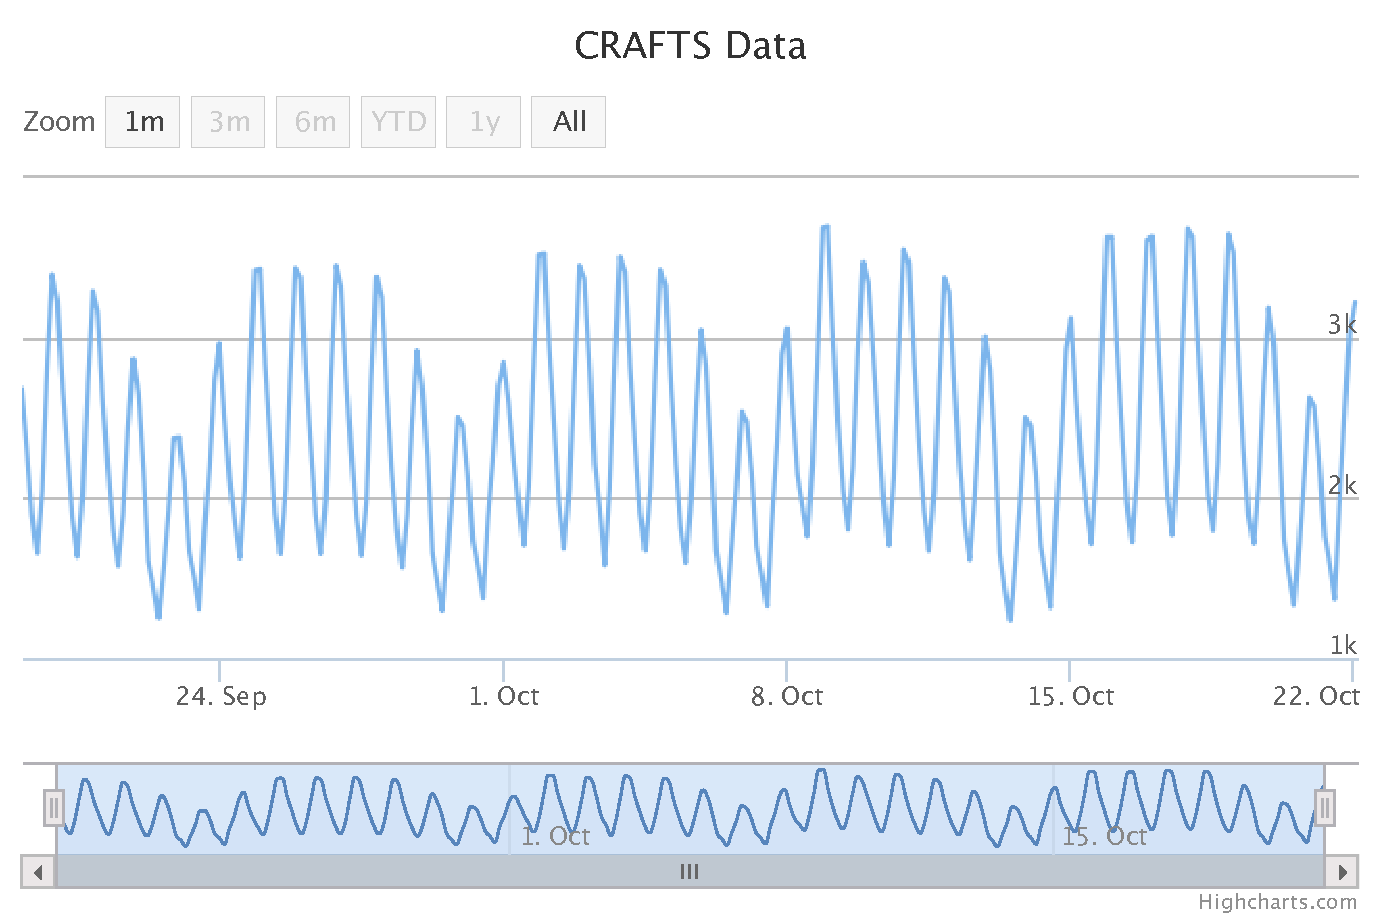
\includegraphics[width=\textwidth]{charts/wikibench.pdf}
\caption{A time-series plot of Wikipedia input data.}
\label{fig:wikibench2}
\end{figure}

This raw Wikipedia workload serves as the baseline for our evaluation. In order to see how our prediction methods are affected by anomalies in the monitoring data, we generated four additional workloads using ARTS' events feature. These workloads introduce outages and usage spikes into the third and fourth weeks of the workload. The third and fourth weeks were chosen because they will be in the training window and prediction horizon, respectively, for our evaluation trials. \Cref{tab:workloads} shows the exact parameters used to generate these workloads and the names by which they will be referred to.

It is important to note that we only use the term ``horizon'' for simplicity. As described in \Cref{ch:policies}, some of our predictors make only short-term predictions, predicting only one point at a time. Anomalies which are present in the ``prediction horizon'' will end up being a part of their training data once the predictor is looking past that point in time.

\begin{table}
\centering
\begin{tabular}{| l | l | l | l | l |}
\hline
Name & Anomaly Type & Start & End & Magnitude \\ \hline
Baseline & none & & & \\ \hline
Training outage & outage & 2007-10-12T17:00 & 2007-10-12T18:00 & \\ \hline
Horizon outage & outage & 2007-10-19T17:00 & 2007-10-19T18:00 & \\ \hline
Training spike & spike & 2007-10-12T17:00 & 2007-10-12T17:15 & 2.0 \\ \hline
Horizon spike & spike & 2007-10-19T17:00 & 2007-10-19T17:15 & 2.0 \\ \hline
\end{tabular}
\caption{ARTS parameters and titles of our evaluation workloads}
\label{tab:workloads}
\end{table}
\chapter{Evaluation}
In order to evaluate the effectiveness of CRAFTS' prediction methods, we run each method on the workloads outlined in \Cref{ch:workloads}. At the beginning of each experiment, the tuner is run on the baseline workload to tune the parameters of the prediction algorithm. This is done to ensure that the tuning is done with minimal anomalies present. Tuning in this way allows us to see how the various algorithms respond to anomalies after an extended period of ``regular'' traffic.

Each predictor will attempt to predict traffic for the week of October 14th in each workload and can use how ever much data it needs before that time for training. The effectiveness of each algorithm is measured using root mean squared deviation (RMSD), as discussed in \Cref{eq:rmsd}. We further break the results down into over-estimations and under-estimations, giving the RMSD for each as well as the percent of predictions which fell into each category. This is done because, in a real-world environment, under-estimations are more costly than over-estimations and we would favor predictors which are more likely to over-estimate than under-estimate. In workloads which contain anomalies, we analyze how the predictor performs during the anomaly separately from how it performs during normal traffic. This allows us to get a more complete view of how a predictor handles anomalies.

In the baseline workload, the goal is to minimize the RMSD for all types. The same is true for regular traffic in all anomalous workloads. For the anomalous training workloads, the predictor should ideally minimize RMSD of all types as well. This result would mean that the anomaly in the training data did not affect the future predictions. In the outage horizon workload, we want to see 100\% over-estimation and maximize over-estimation RMSD during this time. This means that the predictor has successfully ignored the outage. Inversely, we want to see 100\% underestimation and maximize under-estimation RMSD for the spike training workload. These values indicate that the spike was successfully ignored.

The following sections include the evaluation results for each predictor and an analysis of those results. In the graphs below, the light blue line represents the observed data and the black line shows our own predictions.

\section{Translation}
Results for regular traffic show that the translation predictor is prone to underestimation. This is likely due to fluctuations in week by week traffic or a linear trend in the data. In the case of the latter, translation would not be able to account for this since it has no mechanism to account for trends of any kind.

Training data anomalies seriously impact the effectiveness of translation. Since the translation predictor makes no attempt to account for any sort of anomalies, these anomalies are simply preserved and translated into the prediction horizon.

As one would expect, translation is very tolerant to anomalies in the prediction horizon. Since translation makes a long-term prediction, these anomalies won't have an effect on this predictors results until they are part of the training data the next week.

\begin{figure}
\centering
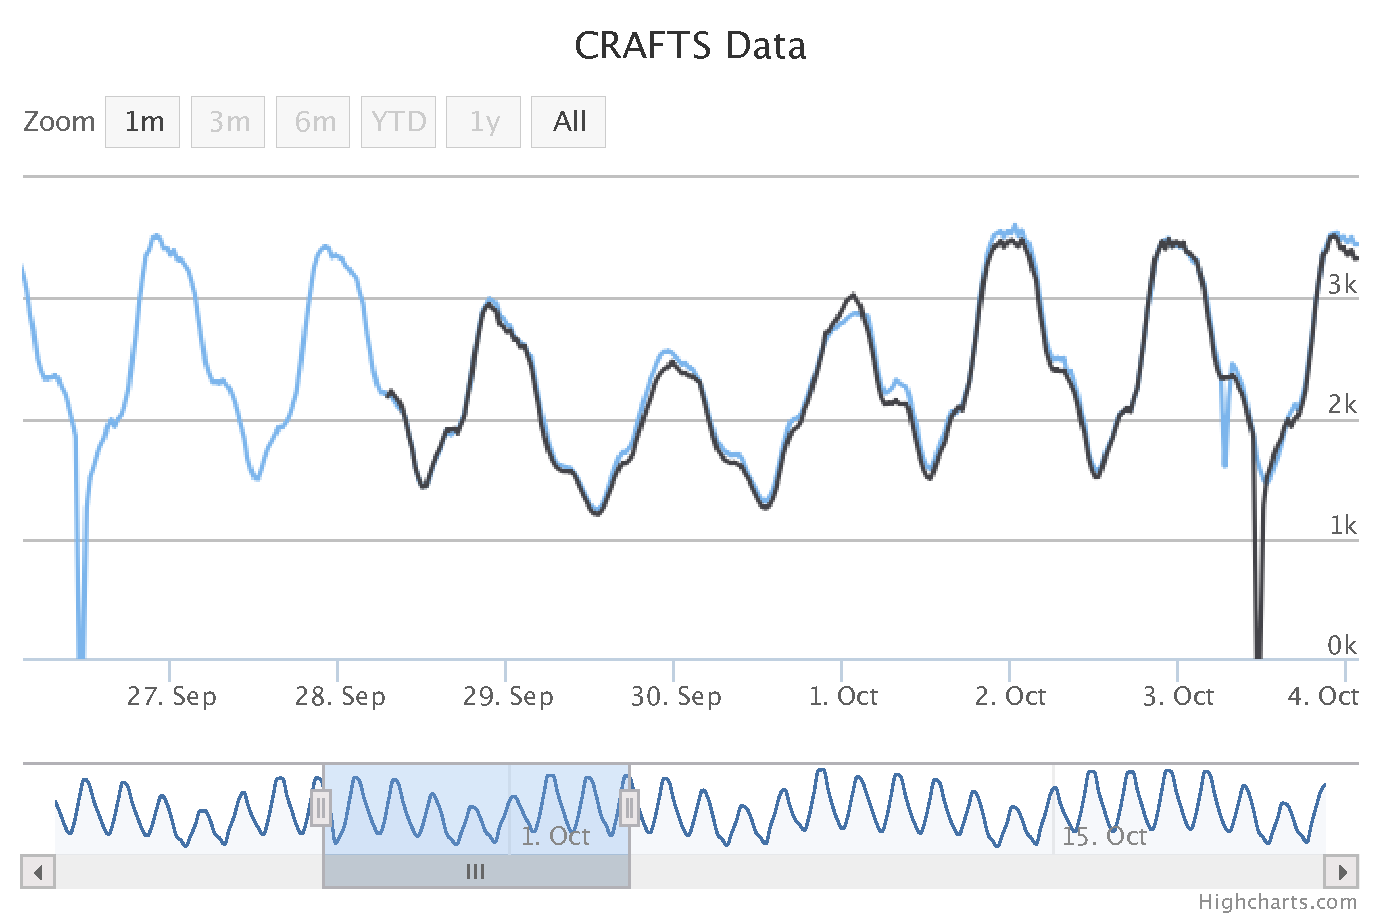
\includegraphics[width=\textwidth]{results/graphs/translation_outage.pdf}
\caption{An outage translated by the translation predictor}
\label{fig:translation_outage}
\end{figure}

\begin{figure}
\centering
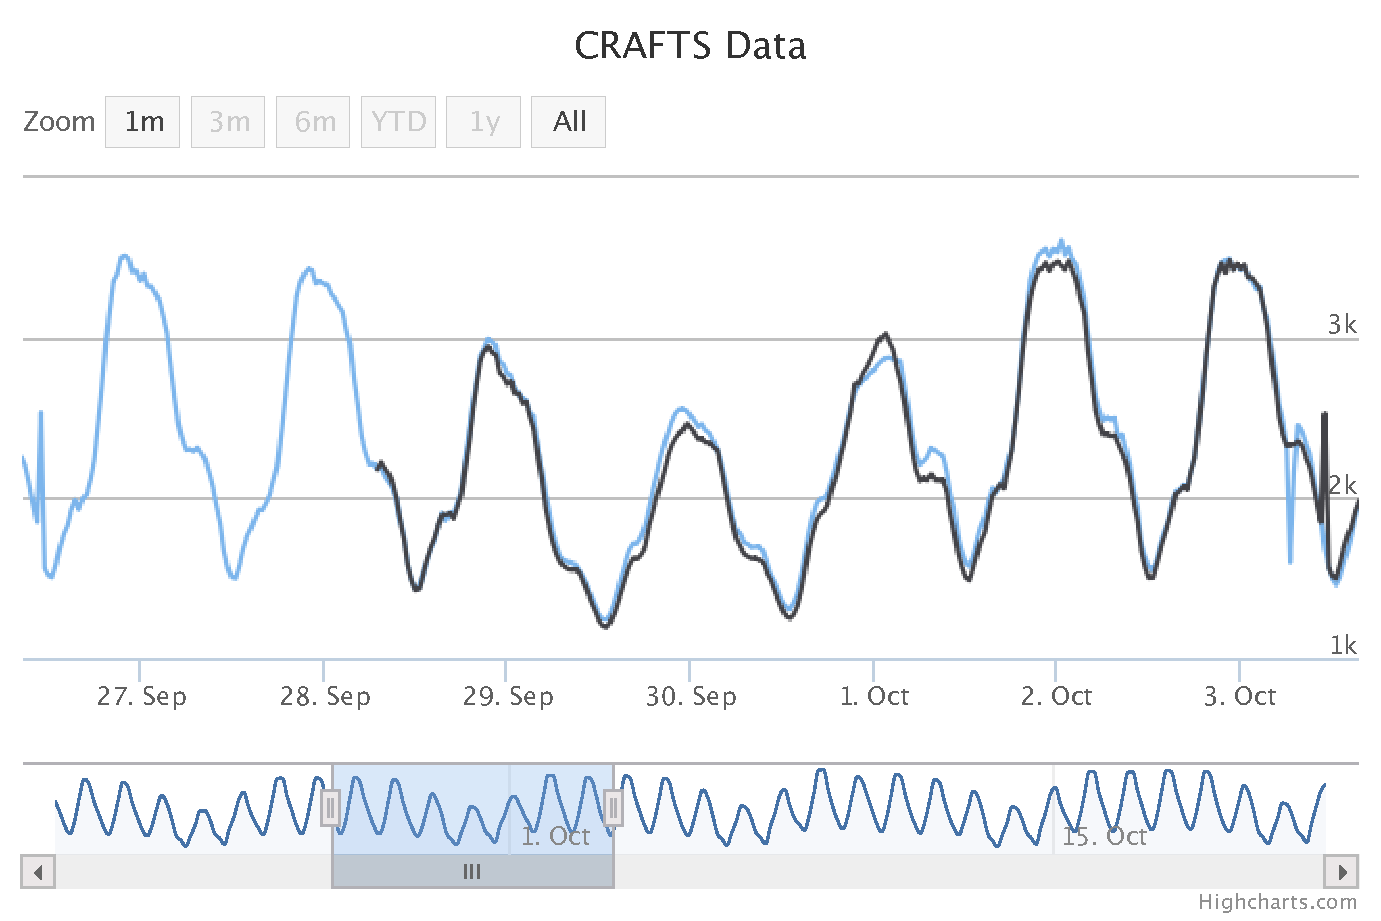
\includegraphics[width=\textwidth]{results/graphs/translation_spike.pdf}
\caption{A usage spike translated by the translation predictor}
\label{fig:translation_spike}
\end{figure}

\begin{table}[H]
\centering
\begin{tabular}{| l | l | l |}
\hline
Type & RMSD & Percent \\ \hline
Under & 113 & 68.7\% \\ \hline
Over & 76 & 31.3\% \\ \hline
Total & 103 & \\ \hline
\end{tabular}
\caption{Translation predictor results for the baseline workload}
\end{table}

% Outage workloads

\begin{table}[H]
\centering
\begin{tabular}{| l | l | l |}
\hline
Type & RMSD & Percent \\ \hline
Under & 122 & 68.7\% \\ \hline
Over & 76 & 31.3\% \\ \hline
Total & 110 & \\ \hline
\end{tabular}
\caption{Translation predictor results for the 10-minute outage workload}
\end{table}

\begin{table}[H]
\centering
\begin{tabular}{| l | l | l |}
\hline
Type & RMSD & Percent \\ \hline
Under & 132 & 68.8\% \\ \hline
Over & 76 & 31.2\% \\ \hline
Total & 117 & \\ \hline
\end{tabular}
\caption{Translation predictor results for the 30-minute outage workload}
\end{table}

\begin{table}[H]
\centering
\begin{tabular}{| l | l | l |}
\hline
Type & RMSD & Percent \\ \hline
Under & 145 & 68.9\% \\ \hline
Over & 76 & 31.1\% \\ \hline
Total & 127 & \\ \hline
\end{tabular}
\caption{Translation predictor results for the 60-minute outage workload}
\end{table}

% Spike workloads

\begin{table}[H]
\centering
\begin{tabular}{| l | l | l |}
\hline
Type & RMSD & Percent \\ \hline
Under & 113 & 68.7\% \\ \hline
Over & 83 & 31.3\% \\ \hline
Total & 105 & \\ \hline
\end{tabular}
\caption{predictor results for the low spike workload}
\end{table}

\begin{table}[H]
\centering
\begin{tabular}{| l | l | l |}
\hline
Type & RMSD & Percent \\ \hline
Under & 113 & 68.7\% \\ \hline
Over & 91 & 31.3\% \\ \hline
Total & 107 & \\ \hline
\end{tabular}
\caption{predictor results for the mid spike workload}
\end{table}

\begin{table}[H]
\centering
\begin{tabular}{| l | l | l |}
\hline
Type & RMSD & Percent \\ \hline
Under & 113 & 68.7\% \\ \hline
Over & 102 & 31.3\% \\ \hline
Total & 110 & \\ \hline
\end{tabular}
\caption{predictor results for the high spike workload}
\end{table}

\section{Fast Fourier Transform}
With an optimized smoothing percentage of 96\%, the FFT predictor performs slightly worse than the translation predictor for regular traffic, but sees a 40\% decrease in error for the training outage and an 87\% decrease in error for the training spike workload. While this is a large improvement, the amount of error we observed for the training anomalies was still higher than expected. In order to further investigate these results, we ran a second evaluation on the training outage workload, this time with 99\% filtering. This time we observed a 58\% decrease in error within the anomaly space over the 96\% smoothing run. We also observed a slight decrease in error for regular traffic as well.

In this case, it seems that the tuner did not perform as we had hoped it to. Since there were no anomalies in the data which the \textsf{tuner} was run on, the optimal smoothing percentage was calculated without being able to take these kinds of anomalies into account. Further analysis of the deficiencies in our \textsf{tuner} implementation can be seen in \Cref{ch:conclusions}.

Similarly to the translation predictor, FFT makes long term decisions, so its predictions are unaffected by anomalies in the prediction horizon.

\begin{table}[H]
\centering
\begin{tabular}{| l | l | l |}
\hline
Type & RMSD & Percent \\ \hline
Under & 140 & 76.2\% \\ \hline
Over & 61 & 23.8\% \\ \hline
Total & 125 & \\ \hline
\end{tabular}
\caption{FFT predictor results for the baseline workload}
\end{table}

\begin{figure}[H]
\centering
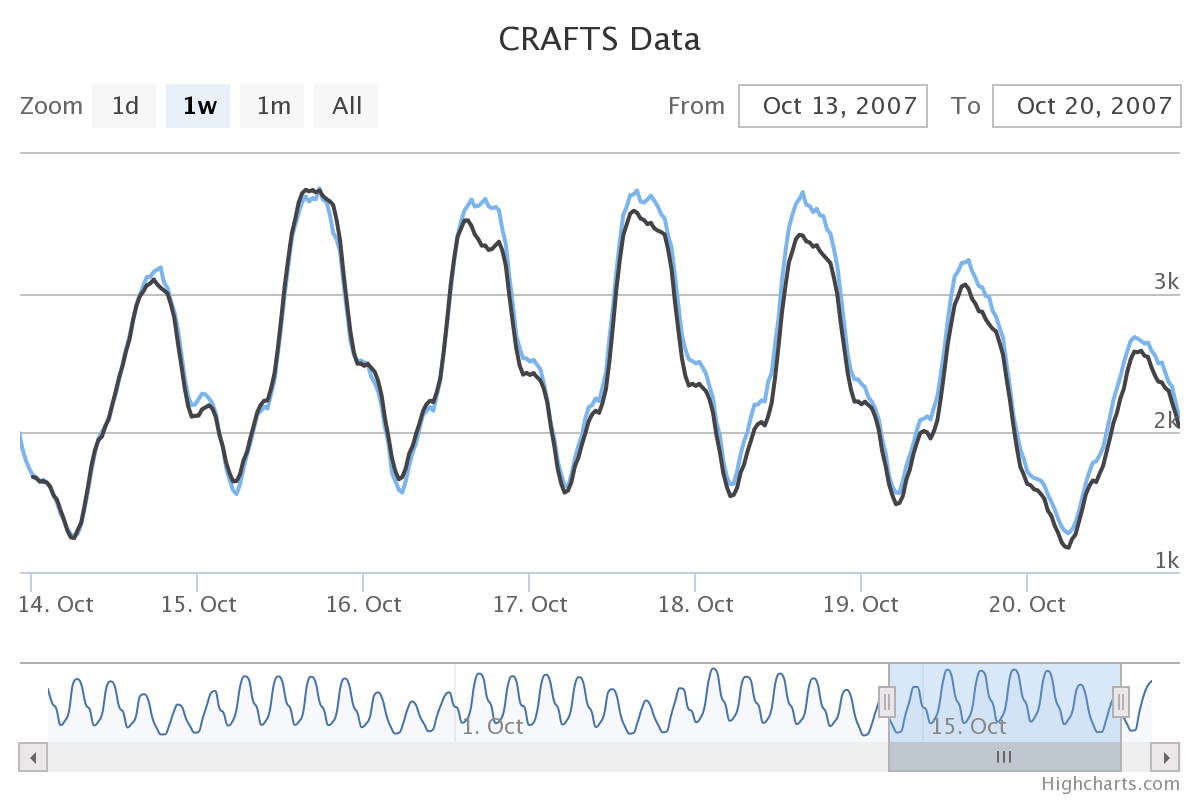
\includegraphics[width=\textwidth]{results/graphs/fft_baseline.png}
\caption{FFT prediction results for the baseline workload}
\label{fig:fft_b}
\end{figure}

\begin{table}[H]
\centering
\begin{tabular}{| l | l | l | l | l |}
\hline
Type & \multicolumn{2}{c |}{Regular} & \multicolumn{2}{c |}{Anomalous} \\ \hline
 & RMSD & Percent & RMSD & Percent \\ \hline
Under & 211 & 74.1\% & 1741 & 100.0\% \\ \hline
Over & 85 & 25.9\% & 0 & 0.0\% \\ \hline
Total & 186 & & 1741 & \\ \hline
\end{tabular}
\caption{FFT predictor results for the training outage workload with 96\% filtering}
\end{table}

\begin{figure}[H]
\centering
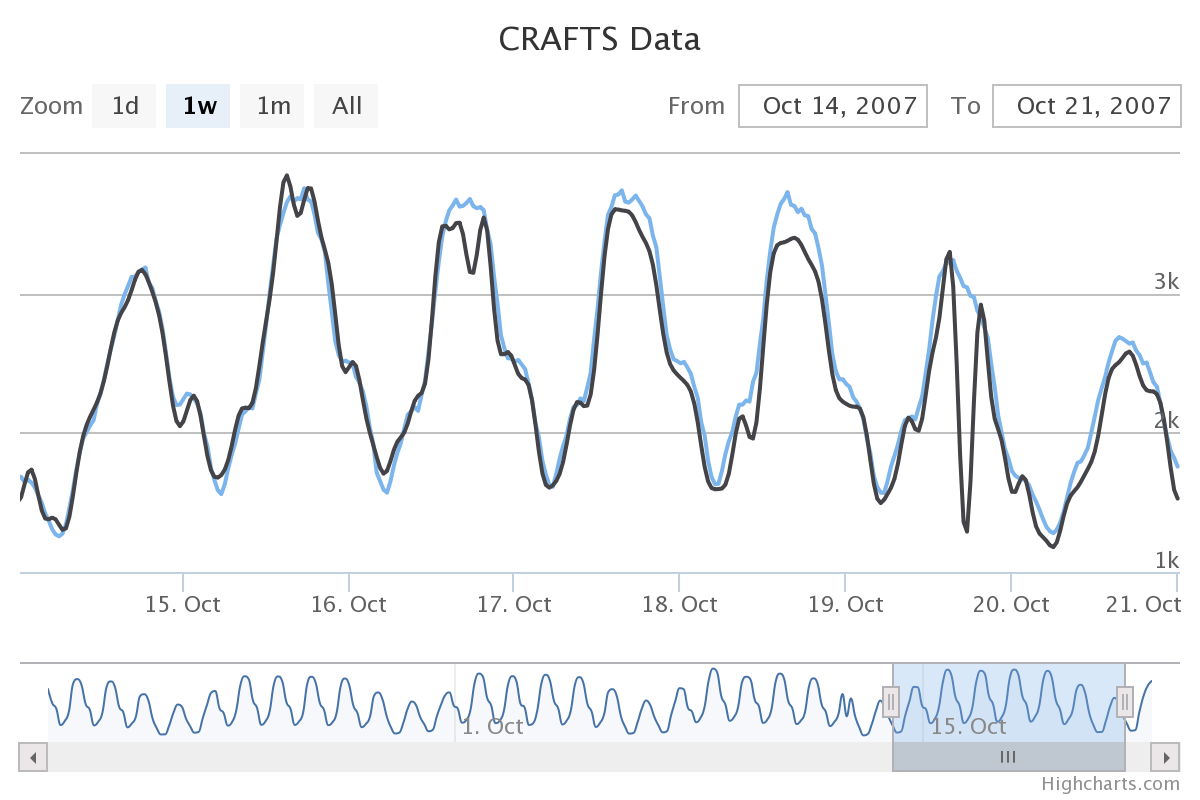
\includegraphics[width=\textwidth]{results/graphs/fft_training_outage_96.png}
\caption{FFT prediction results for the training outage workload with 96\% filtering}
\label{fig:fft_to96}
\end{figure}

\begin{table}[H]
\centering
\begin{tabular}{| l | l | l | l | l |}
\hline
Type & \multicolumn{2}{c |}{Regular} & \multicolumn{2}{c |}{Anomalous} \\ \hline
 & RMSD & Percent & RMSD & Percent \\ \hline
Under & 195 & 75.0\% & 721 & 100.0\% \\ \hline
Over & 88 & 25.0\% & 0 & 0.0\% \\ \hline
Total & 175 & & 721 & \\ \hline
\end{tabular}
\caption{FFT predictor results for the training outage workload with 99\% filtering}
\end{table}

\begin{figure}[H]
\centering
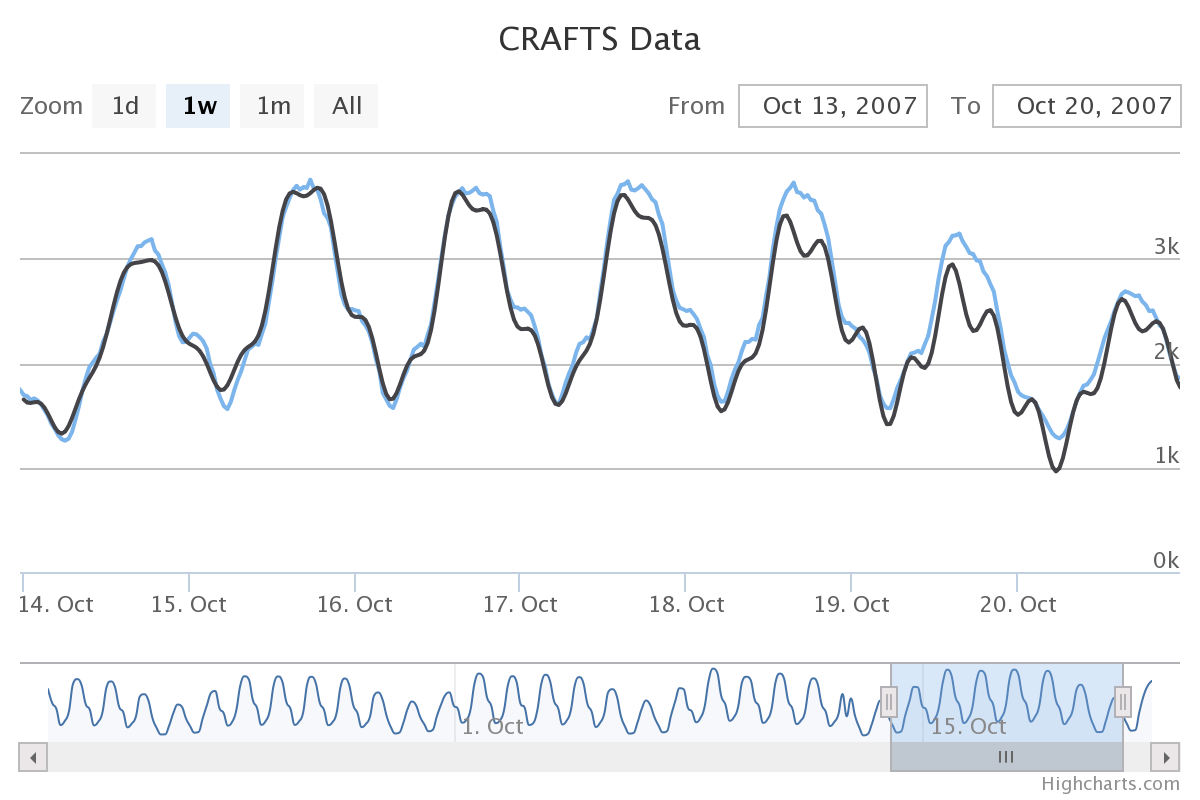
\includegraphics[width=\textwidth]{results/graphs/fft_training_outage_99.png}
\caption{FFT prediction results for the training outage workload with 99\% filtering}
\label{fig:fft_to99}
\end{figure}

\begin{table}[H]
\centering
\begin{tabular}{| l | l | l | l | l |}
\hline
Type & \multicolumn{2}{c |}{Regular} & \multicolumn{2}{c |}{Anomalous} \\ \hline
 & RMSD & Percent & RMSD & Percent \\ \hline
Under & 139 & 75.9\% & 0 & 0.0\% \\ \hline
Over & 194 & 24.1\% & 2869 & 100.0\% \\ \hline
Total & 154 & & 2869 & \\ \hline
\end{tabular}
\caption{FFT predictor results for the horizon outage workload}
\end{table}

\begin{figure}[H]
\centering
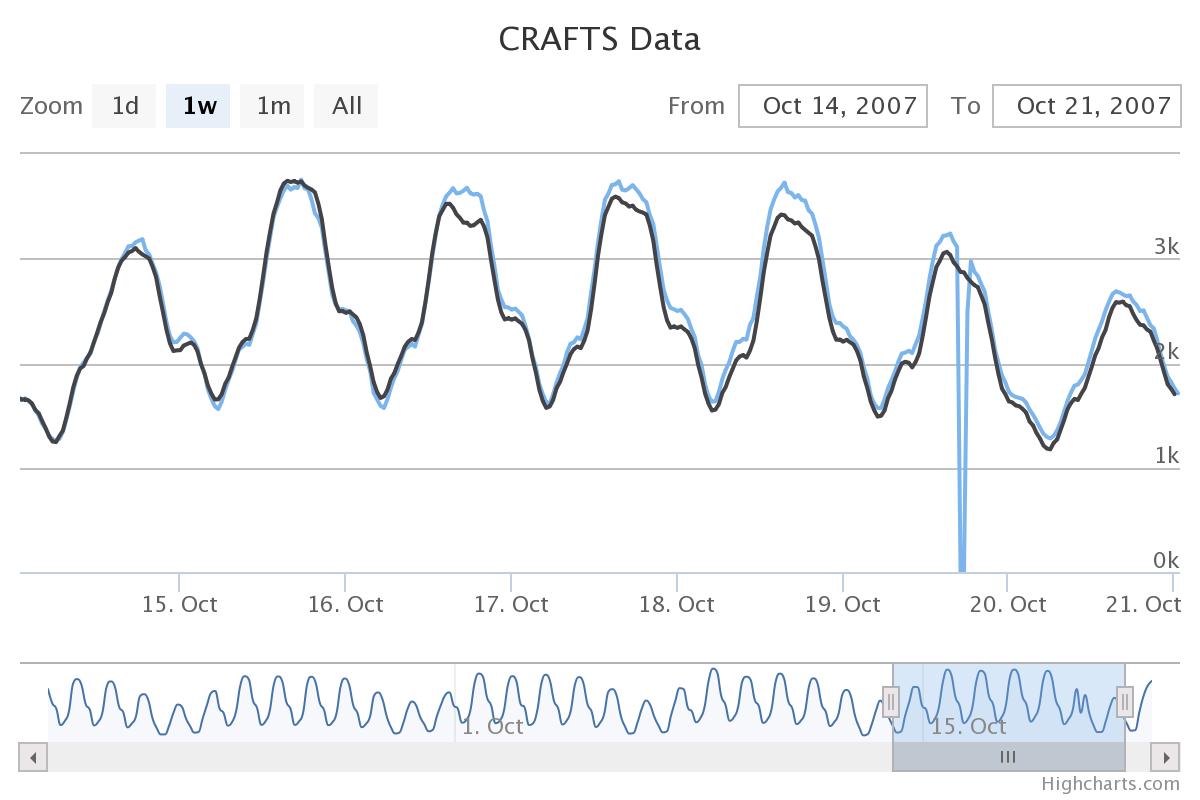
\includegraphics[width=\textwidth]{results/graphs/fft_horizon_outage.png}
\caption{FFT prediction results for the horizon outage workload}
\label{fig:fft_ho}
\end{figure}

\begin{table}[H]
\centering
\begin{tabular}{| l | l | l | l | l |}
\hline
Type & \multicolumn{2}{c |}{Regular} & \multicolumn{2}{c |}{Anomalous} \\ \hline
 & RMSD & Percent & RMSD & Percent \\ \hline
Under & 143 & 74.6\% & 0 & 0.0\% \\ \hline
Over & 86 & 25.4\% & 427 & 100.0\% \\ \hline
Total & 131 & & 427 & \\ \hline
\end{tabular}
\caption{FFT predictor results for the training spike workload}
\end{table}

\begin{figure}[H]
\centering
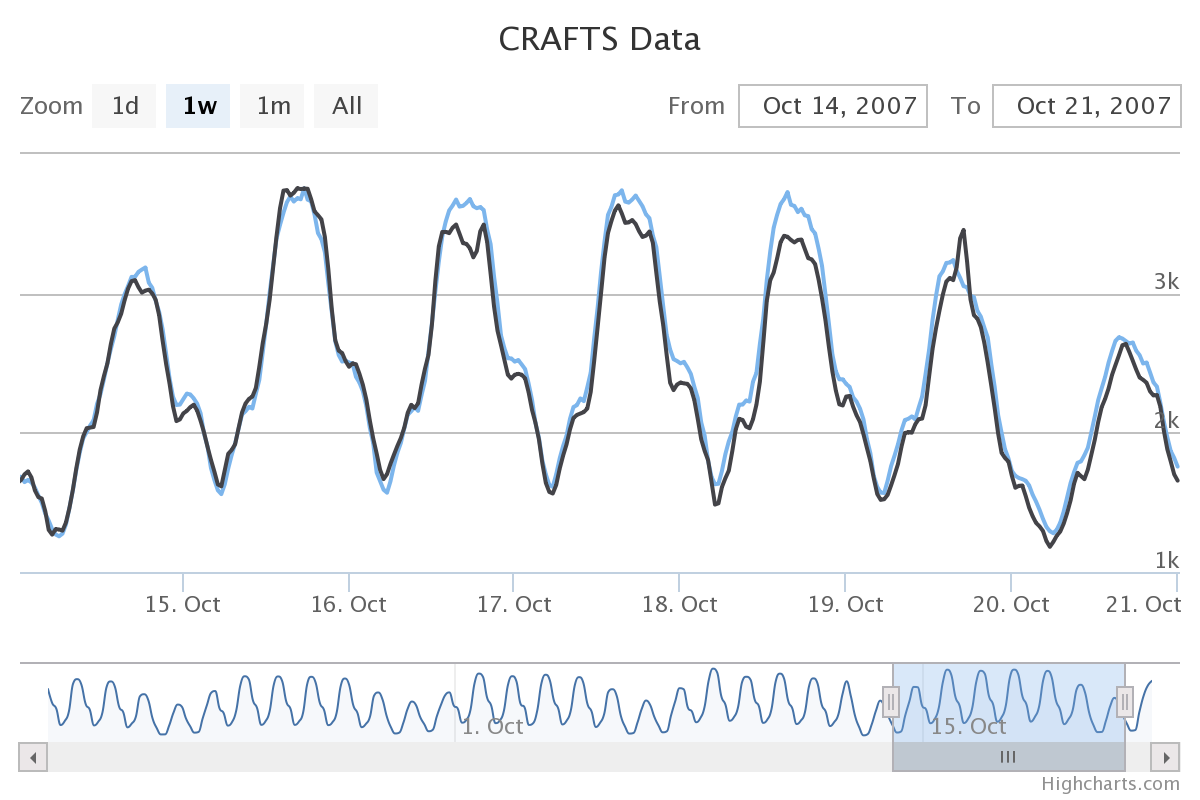
\includegraphics[width=\textwidth]{results/graphs/fft_training_spike.png}
\caption{FFT prediction results for the training spike workload}
\label{fig:fft_ts}
\end{figure}

\begin{table}[H]
\centering
\begin{tabular}{| l | l | l | l | l |}
\hline
Type & \multicolumn{2}{c |}{Regular} & \multicolumn{2}{c |}{Anomalous} \\ \hline
 & RMSD & Percent & RMSD & Percent \\ \hline
Under & 181 & 76.1\% & 3239 & 100.0\% \\ \hline
Over & 61 & 23.9\% & 0 & 0.0\% \\ \hline
Total & 161 & & 3239 & \\ \hline
\end{tabular}
\caption{FFT predictor results for the horizon spike workload}
\end{table}

\begin{figure}[H]
\centering
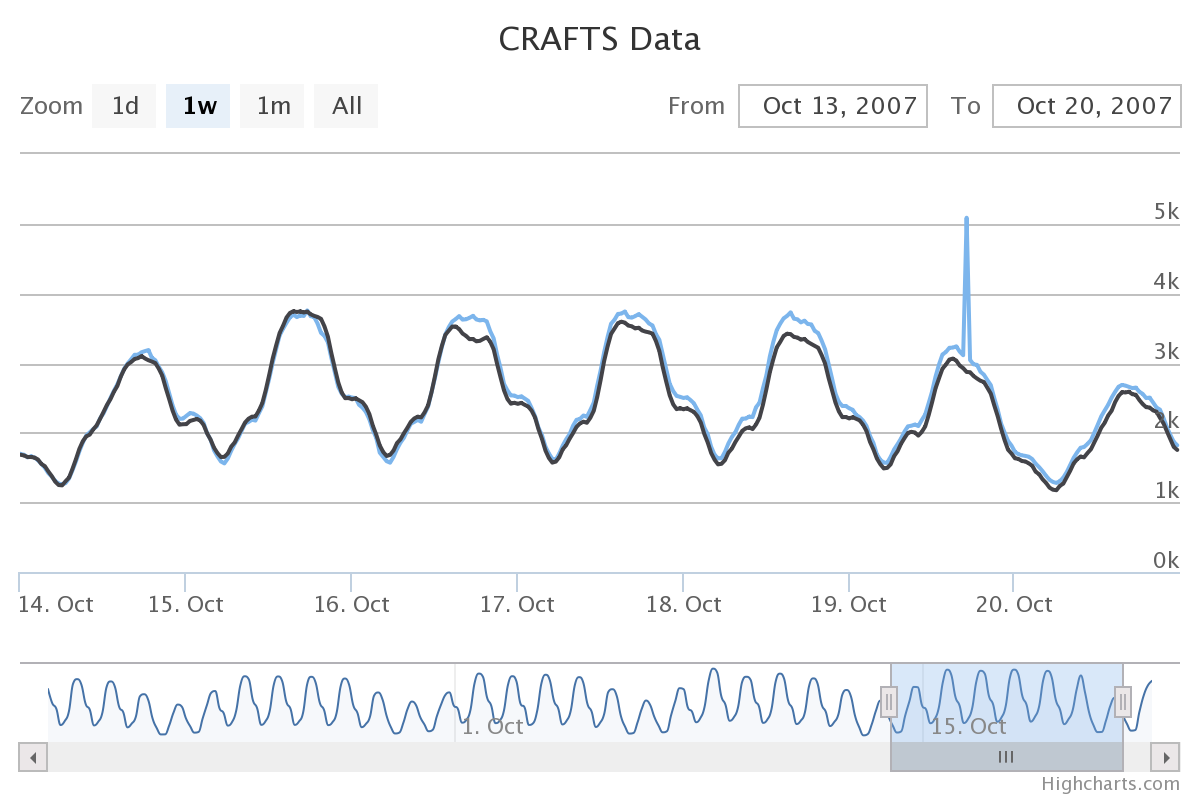
\includegraphics[width=\textwidth]{results/graphs/fft_horizon_spike.png}
\caption{FFT prediction results for the horizon spike workload}
\label{fig:fft_hs}
\end{figure}

\section{Linear Regression}
Linear regression performs neck and neck with the translation baseline for regular traffic, but truly shines when presented with training anomalies. Since the Thiel-Sen estimator is tolerant to outliers, the anomalies present in the training data are largely ignored. We observe RMSD values within the anomaly space smaller than any predictor evaluated thus far.

Again, as a long-term predictor, anomalies in the prediction horizon have no effect on the linear regression predictor's effectiveness.

\begin{table}[H]
\centering
\begin{tabular}{| l | l | l |}
\hline
Type & RMSD & Percent \\ \hline
Under & 138 & 89.2\% \\ \hline
Over & 32 & 10.8\% \\ \hline
Total & 131 & \\ \hline
\end{tabular}
\caption{Regression predictor results for the baseline workload}
\end{table}

\begin{figure}[H]
\centering
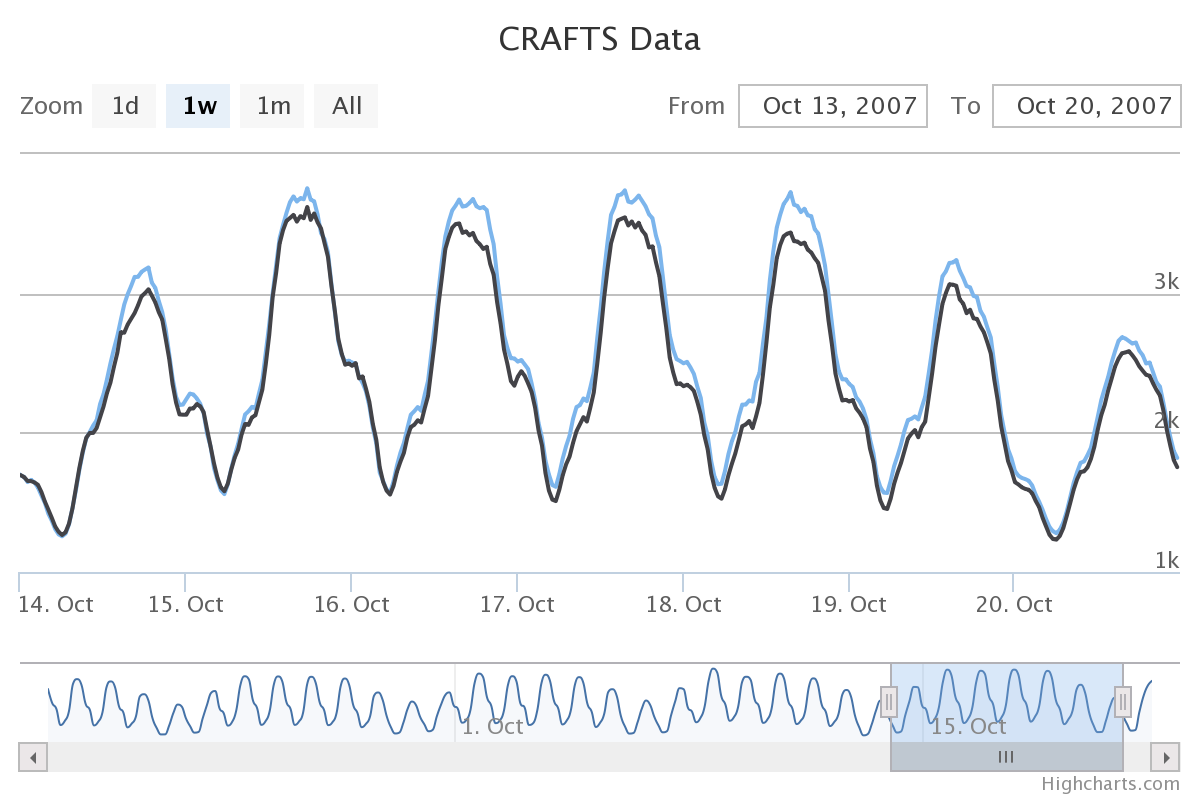
\includegraphics[width=\textwidth]{results/graphs/regression_baseline.png}
\caption{Regression prediction results for the baseline workload}
\label{fig:regression_b}
\end{figure}

\begin{table}[H]
\centering
\begin{tabular}{| l | l | l | l | l |}
\hline
Type & \multicolumn{2}{c |}{Regular} & \multicolumn{2}{c |}{Anomalous} \\ \hline
 & RMSD & Percent & RMSD & Percent \\ \hline
Under & 138 & 89.1\% & 270 & 100.0\% \\ \hline
Over & 32 & 10.9\% & 0 & 0.0\% \\ \hline
Total & 131 & & 270 & \\ \hline
\end{tabular}
\caption{Regression predictor results for the training outage workload}
\end{table}

\begin{figure}[H]
\centering
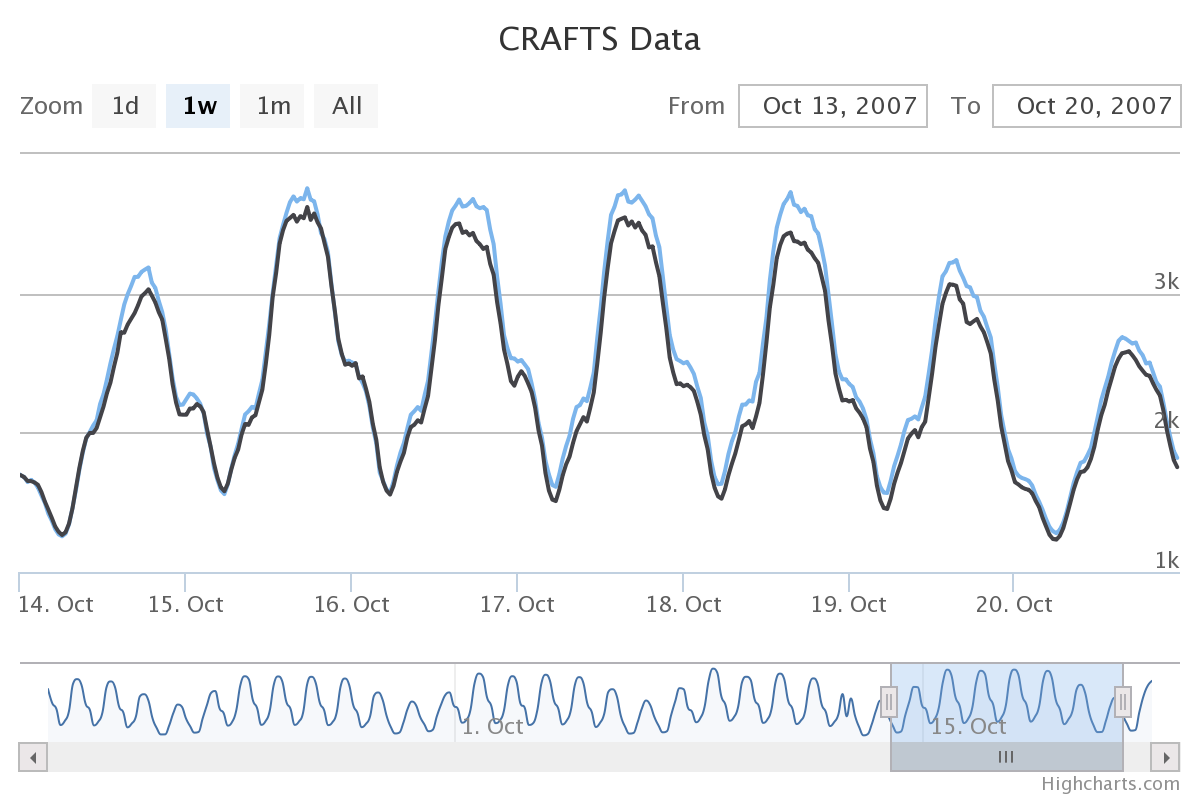
\includegraphics[width=\textwidth]{results/graphs/regression_training_outage.png}
\caption{Regression prediction results for the training outage workload}
\label{fig:regression_to}
\end{figure}

\begin{table}[H]
\centering
\begin{tabular}{| l | l | l | l | l |}
\hline
Type & \multicolumn{2}{c |}{Regular} & \multicolumn{2}{c |}{Anomalous} \\ \hline
 & RMSD & Percent & RMSD & Percent \\ \hline
Under & 138 & 89.0\% & 0 & 0.0\% \\ \hline
Over & 274 & 11.0\% & 2869 & 100.0\% \\ \hline
Total & 159 & & 2869 & \\ \hline
\end{tabular}
\caption{Regression predictor results for the horizon outage workload}
\end{table}

\begin{figure}[H]
\centering
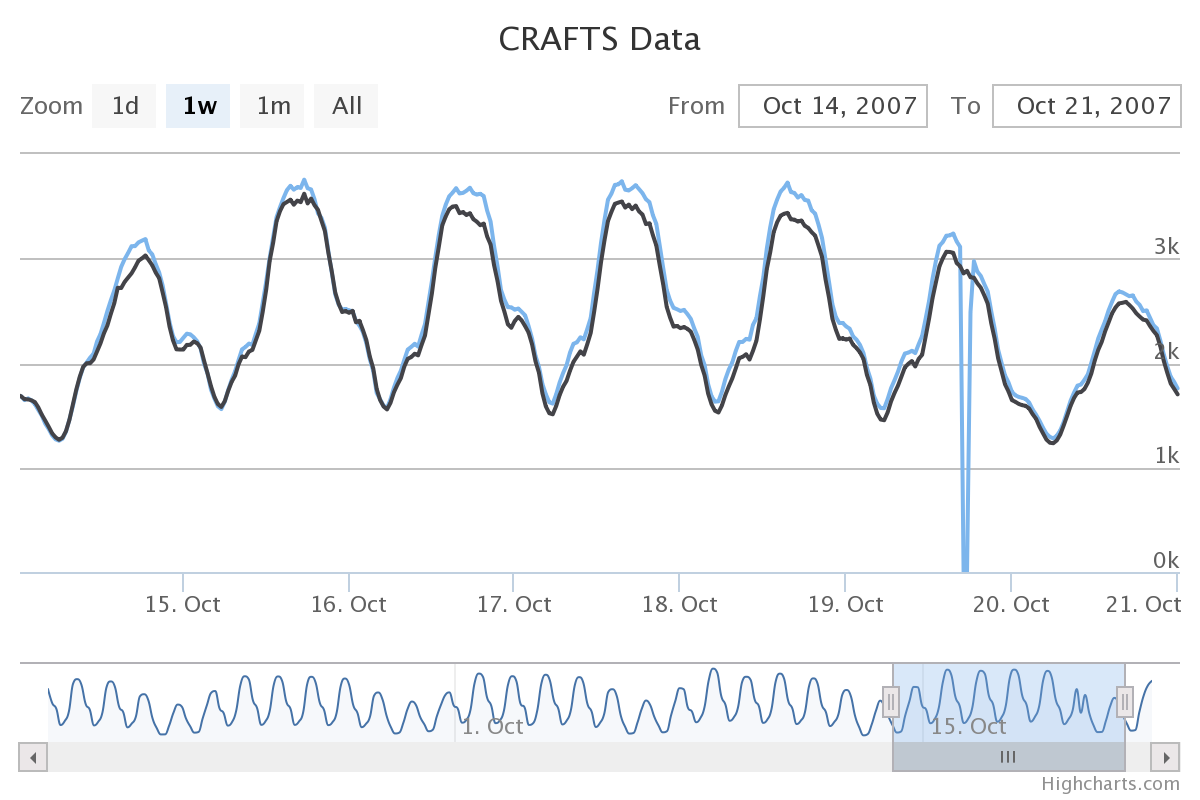
\includegraphics[width=\textwidth]{results/graphs/regression_horizon_outage.png}
\caption{Regression prediction results for the horizon outage workload}
\label{fig:regression_ho}
\end{figure}

\begin{table}[H]
\centering
\begin{tabular}{| l | l | l | l | l |}
\hline
Type & \multicolumn{2}{c |}{Regular} & \multicolumn{2}{c |}{Anomalous} \\ \hline
 & RMSD & Percent & RMSD & Percent \\ \hline
Under & 138 & 89.2\% & 177 & 100.0\% \\ \hline
Over & 32 & 10.8\% & 0 & 0.0\% \\ \hline
Total & 131 & & 177 & \\ \hline
\end{tabular}
\caption{Regression predictor results for the training spike workload}
\end{table}

\begin{figure}[H]
\centering
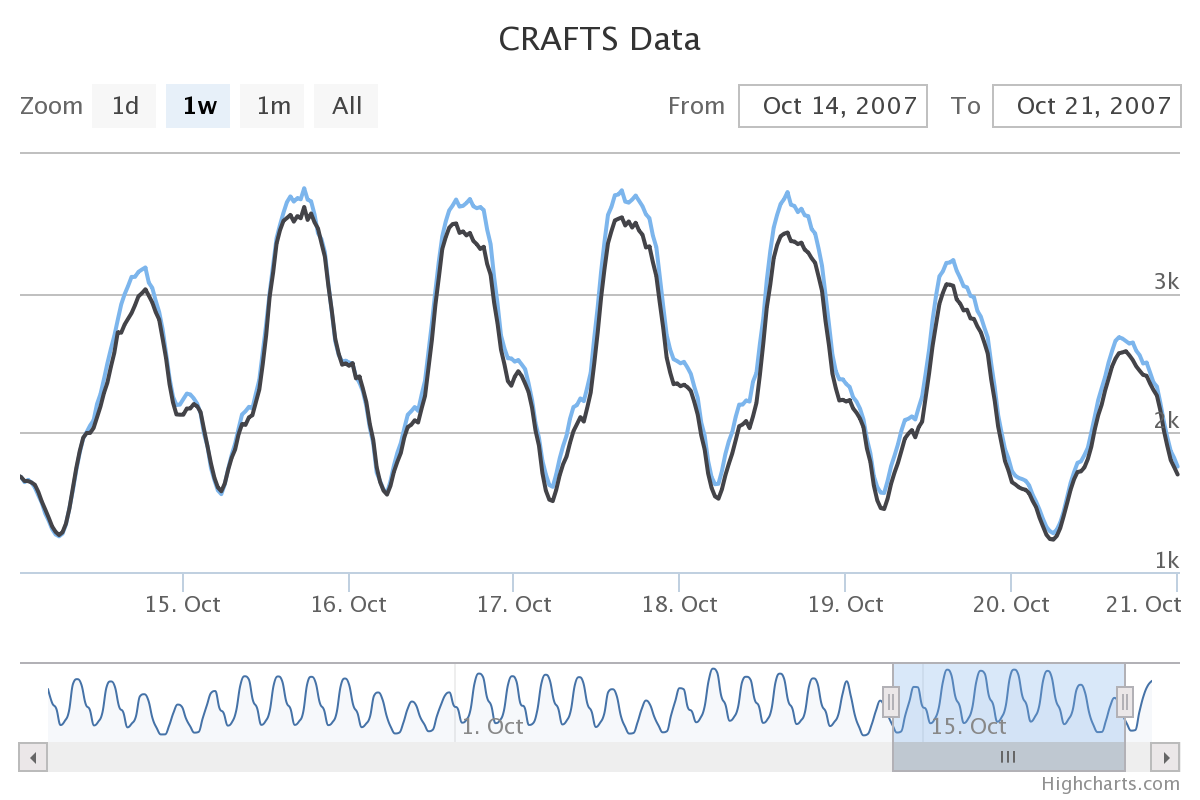
\includegraphics[width=\textwidth]{results/graphs/regression_training_spike.png}
\caption{Regression prediction results for the training spike workload}
\label{fig:regression_ts}
\end{figure}

\begin{table}[H]
\centering
\begin{tabular}{| l | l | l | l | l |}
\hline
Type & \multicolumn{2}{c |}{Regular} & \multicolumn{2}{c |}{Anomalous} \\ \hline
 & RMSD & Percent & RMSD & Percent \\ \hline
Under & 175 & 89.2\% & 3260 & 100.0\% \\ \hline
Over & 32 & 10.8\% & 0 & 0.0\% \\ \hline
Total & 166 & & 3260 & \\ \hline
\end{tabular}
\caption{Regression predictor results for the horizon spike workload}
\end{table}

\begin{figure}[H]
\centering
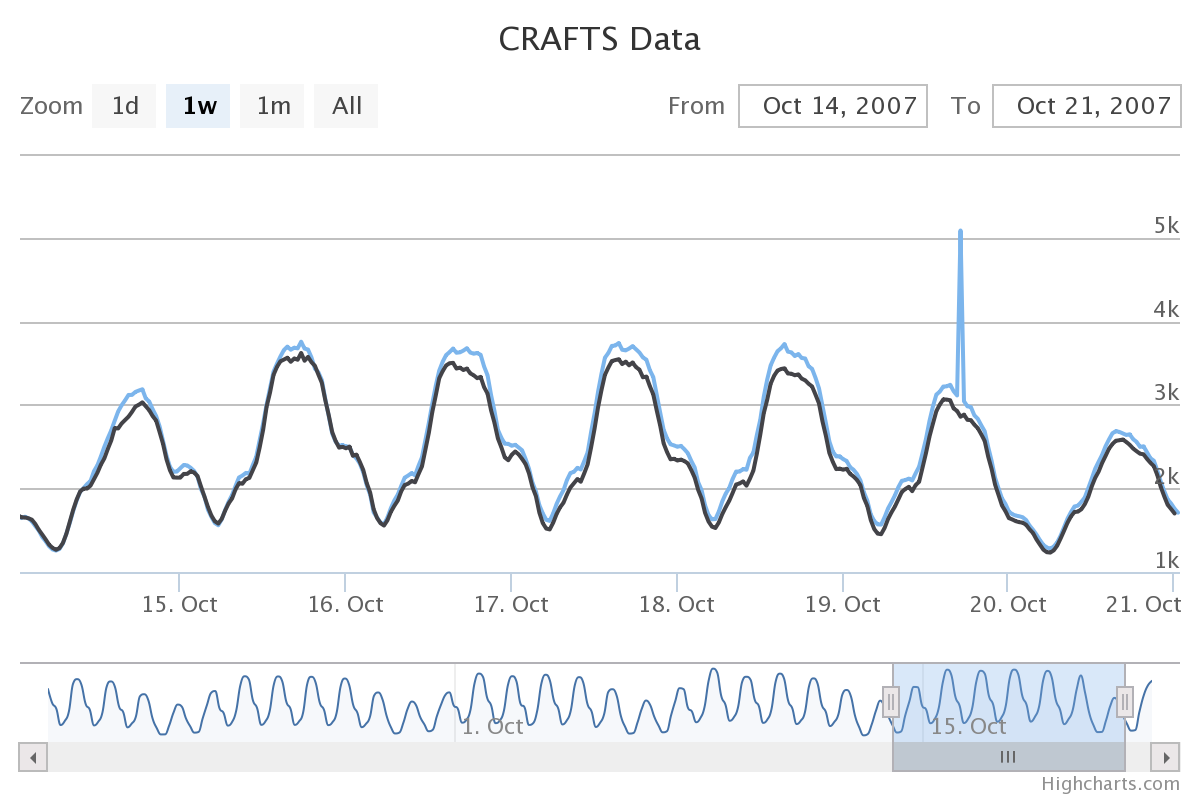
\includegraphics[width=\textwidth]{results/graphs/regression_horizon_spike.png}
\caption{Regression prediction results for the horizon spike workload}
\label{fig:regression_hs}
\end{figure}

\section{Discrete-Time Markov Chain}
The Markov predictor produced the best results for most regular traffic scenarios we have seen so far, but as seen in \Cref{fig:markov_b,fig:markov_ho,fig:markov_ts,fig:markov_hs}, there are some peculiar anomalies present in its predictions. These sudden dips can likely be attributed to the periodic nature of the data. Since the transition probability matrix is based on the likelihood of moving between one bucket and another bucket, a perfect sine wave would produce a transition probability matrix where it is equally likely to move to a higher bucket or a lower bucket. Similarly, since our data is periodic, it is likely that in some cases the probability of moving to a lower bucket is more likely than moving to a higher bucket, even if there is an upwards trend in the observations.

The Markov predictor is also very sensitive to anomalies in the prediction horizon. Since this predictor makes predictions only a short amount of time into the future, it is likely that a prediction will be made while an anomaly is occurring and be used as the base observation in the transition probability matrix.

The short-term nature of this predictor also has repercussions on the \textsf{planner's} ability to do its job properly. This will be discussed further in \Cref{ch:conclusions}.

\begin{table}[H]
\centering
\begin{tabular}{| l | l | l | l | l | l |}
\hline
Type & RMSD & Percent \\ \hline
Under & 27 & 74.0\% \\ \hline
Over & 22 & 26.0\% \\ \hline
Total & 26 & \\ \hline
\end{tabular}
\caption{Markov predictor results for the baseline workload}
\end{table}

% Outage workloads

\begin{table}[H]
\centering
\begin{tabular}{| l | l | l |}
\hline
Type & RMSD & Percent \\ \hline
Under & 52 & 80.8\% \\ \hline
Over & 39 & 19.2\% \\ \hline
Total & 50 & \\ \hline
\end{tabular}
\caption{predictor results for the 10-minute outage workload}
\end{table}

\begin{table}[H]
\centering
\begin{tabular}{| l | l | l |}
\hline
Type & RMSD & Percent \\ \hline
Under & 52 & 80.9\% \\ \hline
Over & 40 & 19.1\% \\ \hline
Total & 50 & \\ \hline
\end{tabular}
\caption{predictor results for the 30-minute outage workload}
\end{table}

\begin{table}[H]
\centering
\begin{tabular}{| l | l | l |}
\hline
Type & RMSD & Percent \\ \hline
Under & 52 & 80.9\% \\ \hline
Over & 39 & 19.1\% \\ \hline
Total & 50 & \\ \hline
\end{tabular}
\caption{predictor results for the 60-minute outage workload}
\end{table}

% Spike workloads

\begin{table}[H]
\centering
\begin{tabular}{| l | l | l |}
\hline
Type & RMSD & Percent \\ \hline
Under & 48 & 76.9\% \\ \hline
Over & 39 & 23.1\% \\ \hline
Total & 46 & \\ \hline
\end{tabular}
\caption{predictor results for the low spike workload}
\end{table}

\begin{table}[H]
\centering
\begin{tabular}{| l | l | l |}
\hline
Type & RMSD & Percent \\ \hline
Under & 48 & 76.9\% \\ \hline
Over & 38 & 23.1\% \\ \hline
Total & 46 & \\ \hline
\end{tabular}
\caption{predictor results for the mid spike workload}
\end{table}

\begin{table}[H]
\centering
\begin{tabular}{| l | l | l |}
\hline
Type & RMSD & Percent \\ \hline
Under & 48 & 76.9\% \\ \hline
Over & 38 & 23.1\% \\ \hline
Total & 46 & \\ \hline
\end{tabular}
\caption{predictor results for the high spike workload}
\end{table}

\section{Exponential Smoothing}
While exponential smoothing produces results for regular traffic which are on par with the Markov predictor, exponential smoothing does not suffer from the anomalies seen in the Markov predictions.

In the anomalous horizon workloads, we can see that not only does the prediction curve follow the anomalies, it also displays a ``bouncing'' effect. Since the goal of exponential smoothing is to produce a smooth curve, the quick turnaround when recovering from an outage of spike causes the prediction data to bounce before returning to a desirable state.

Due to its short-term nature, exponential smoothing also suffers from the same issues present in the Markov predictor. Again, these issues will be discussed in \Cref{ch:conclusions}.

\begin{table}[H]
\centering
\begin{tabular}{| l | l | l |}
\hline
Type & RMSD & Percent \\ \hline
Under & 42 & 53.2\% \\ \hline
Over & 48 & 46.8\% \\ \hline
Total & 45 & \\ \hline
\end{tabular}
\caption{Exponential smoothing predictor results for the baseline workload}
\end{table}

\begin{figure}[H]
\centering
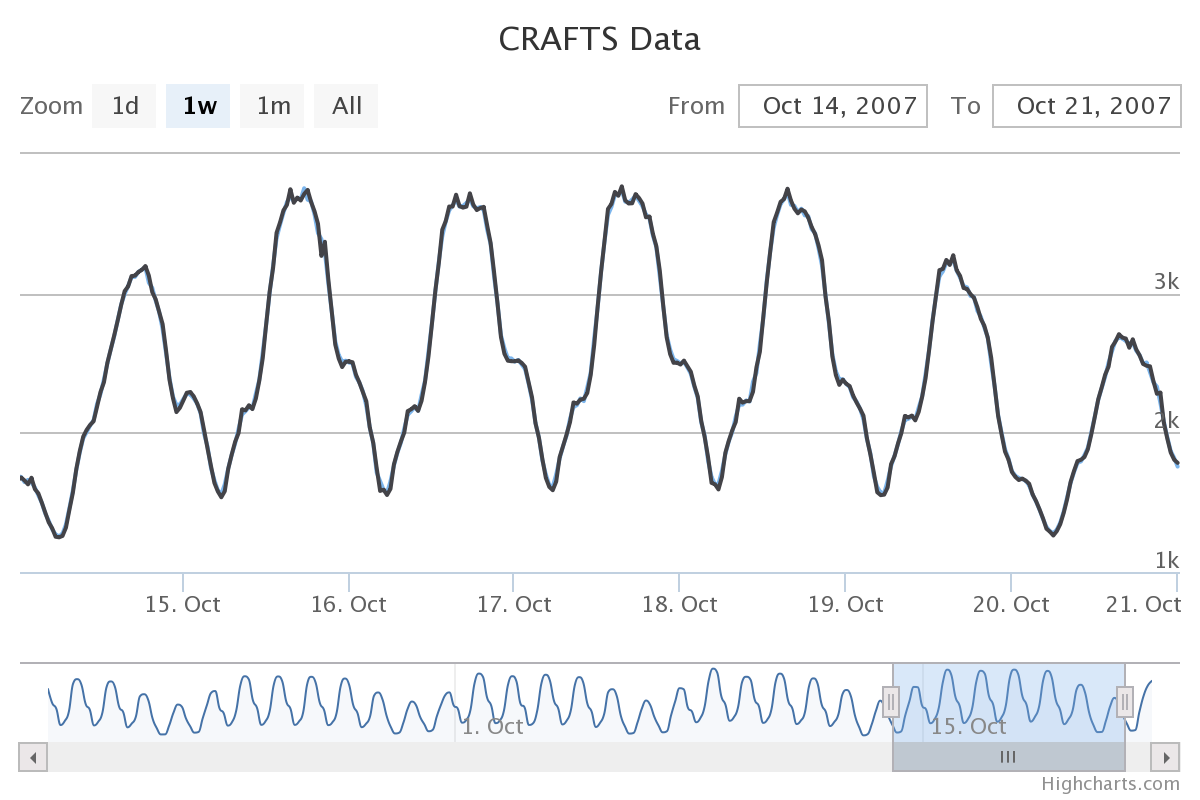
\includegraphics[width=\textwidth]{results/graphs/smoothing_baseline.png}
\caption{Exponential smoothing prediction results for the baseline workload}
\label{fig:smoothing_b}
\end{figure}

\begin{table}[H]
\centering
\begin{tabular}{| l | l | l | l | l |}
\hline
Type & \multicolumn{2}{c |}{Regular} & \multicolumn{2}{c |}{Anomalous} \\ \hline
 & RMSD & Percent & RMSD & Percent \\ \hline
Under & 42 & 53.1\% & 31 & 72.7\% \\ \hline
Over & 48 & 46.9\% & 22 & 27.3\% \\ \hline
Total & 45 & & 29 & \\ \hline
\end{tabular}
\caption{Exponential smoothing predictor results for the training outage workload}
\end{table}

\begin{figure}[H]
\centering
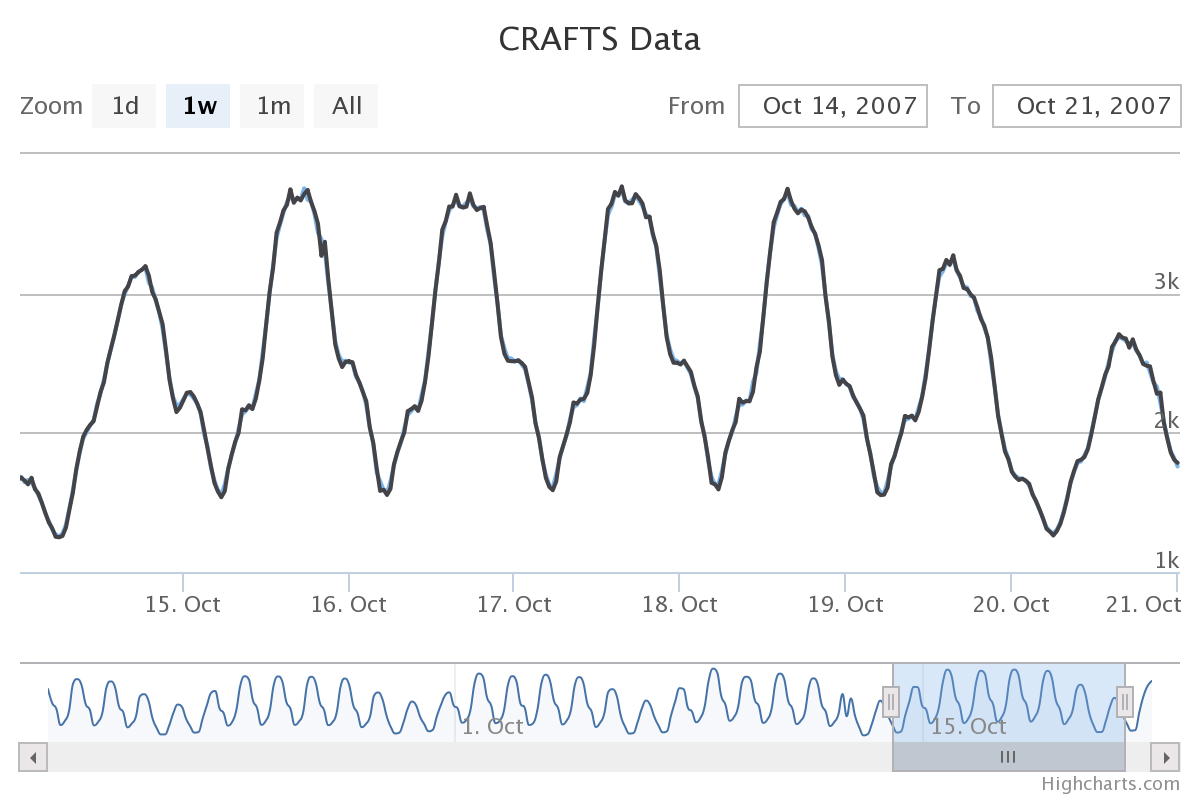
\includegraphics[width=\textwidth]{results/graphs/smoothing_training_outage.png}
\caption{Exponential smoothing prediction results for the training outage workload}
\label{fig:smoothing_to}
\end{figure}

\begin{table}[H]
\centering
\begin{tabular}{| l | l | l | l | l |}
\hline
Type & \multicolumn{2}{c |}{Regular} & \multicolumn{2}{c |}{Anomalous} \\ \hline
 & RMSD & Percent & RMSD & Percent \\ \hline
Under & 165 & 53.0\% & 1216 & 81.8\% \\ \hline
Over & 159 & 47.0\% & 3068 & 18.2\% \\ \hline
Total & 162 & & 1709 & \\ \hline
\end{tabular}
\caption{Exponential smoothing predictor results for the horizon outage workload}
\end{table}

\begin{figure}[H]
\centering
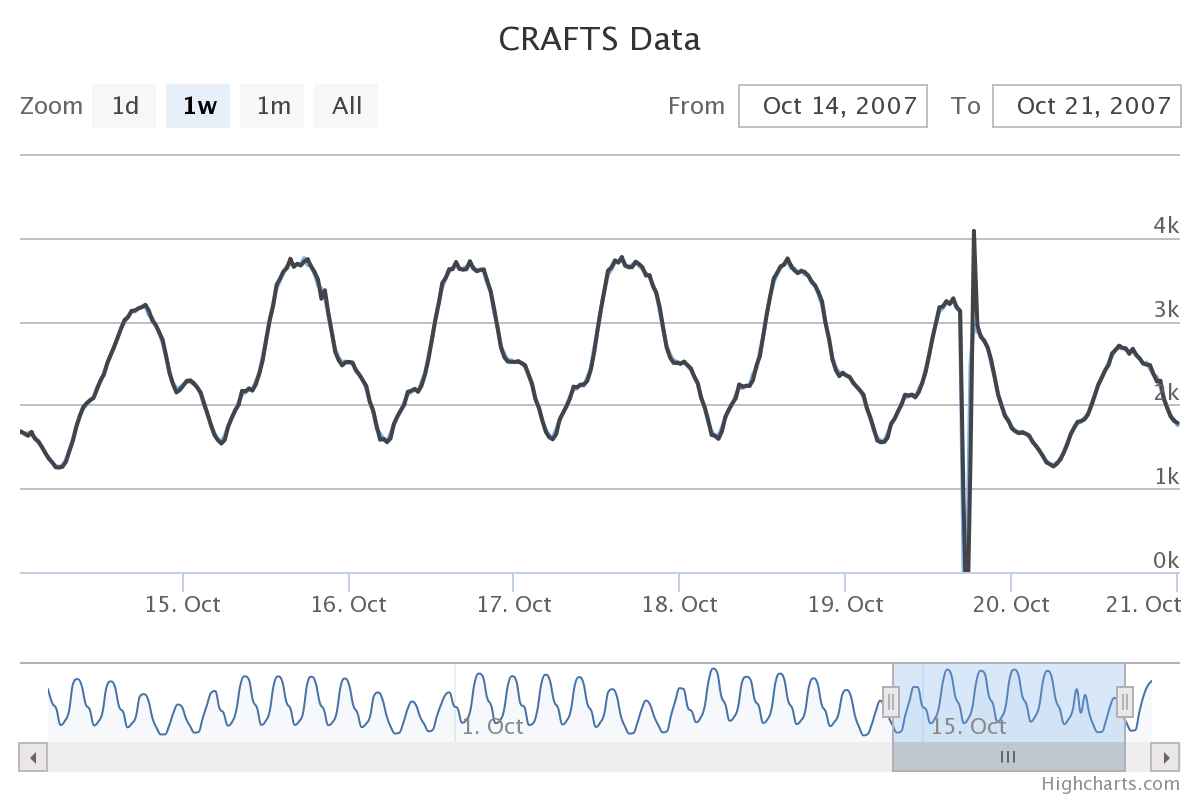
\includegraphics[width=\textwidth]{results/graphs/smoothing_horizon_outage.png}
\caption{Exponential smoothing prediction results for the horizon outage workload}
\label{fig:smoothing_ho}
\end{figure}

\begin{table}[H]
\centering
\begin{tabular}{| l | l | l | l | l |}
\hline
Type & \multicolumn{2}{c |}{Regular} & \multicolumn{2}{c |}{Anomalous} \\ \hline
 & RMSD & Percent & RMSD & Percent \\ \hline
Under & 42 & 53.2\% & 0 & 0.0\% \\ \hline
Over & 48 & 46.8\% & 16 & 100.0\% \\ \hline
Total & 45 & & 16 & \\ \hline
\end{tabular}
\caption{Exponential smoothing predictor results for the training spike workload}
\end{table}

\begin{figure}[H]
\centering
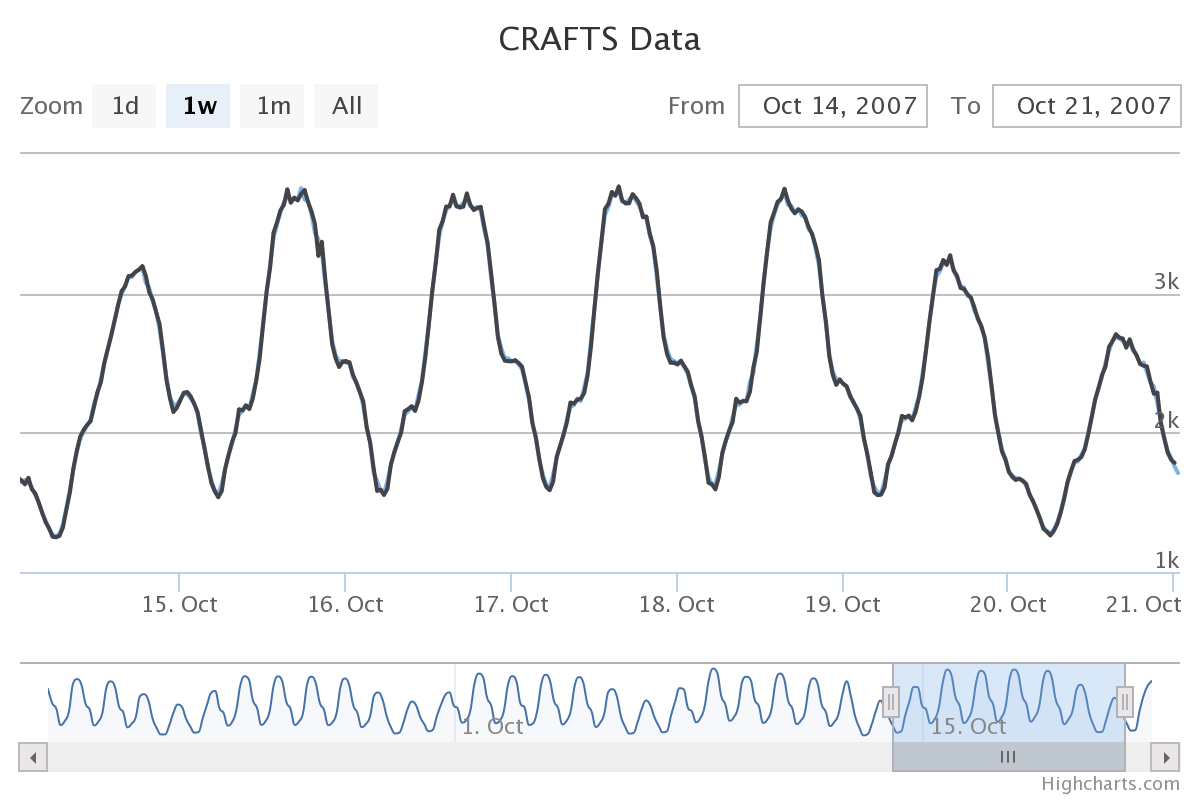
\includegraphics[width=\textwidth]{results/graphs/smoothing_training_spike.png}
\caption{Exponential smoothing prediction results for the training spike workload}
\label{fig:smoothing_ts}
\end{figure}

\begin{table}[H]
\centering
\begin{tabular}{| l | l | l | l | l |}
\hline
Type & \multicolumn{2}{c |}{Regular} & \multicolumn{2}{c |}{Anomalous} \\ \hline
 & RMSD & Percent & RMSD & Percent \\ \hline
Under & 129 & 53.2\% & 3036 & 100.0\% \\ \hline
Over & 277 & 46.8\% & 0 & 0.0\% \\ \hline
Total & 212 & & 3036 & \\ \hline
\end{tabular}
\caption{Exponential smoothing predictor results for the horizon spike workload}
\end{table}

\begin{figure}[H]
\centering
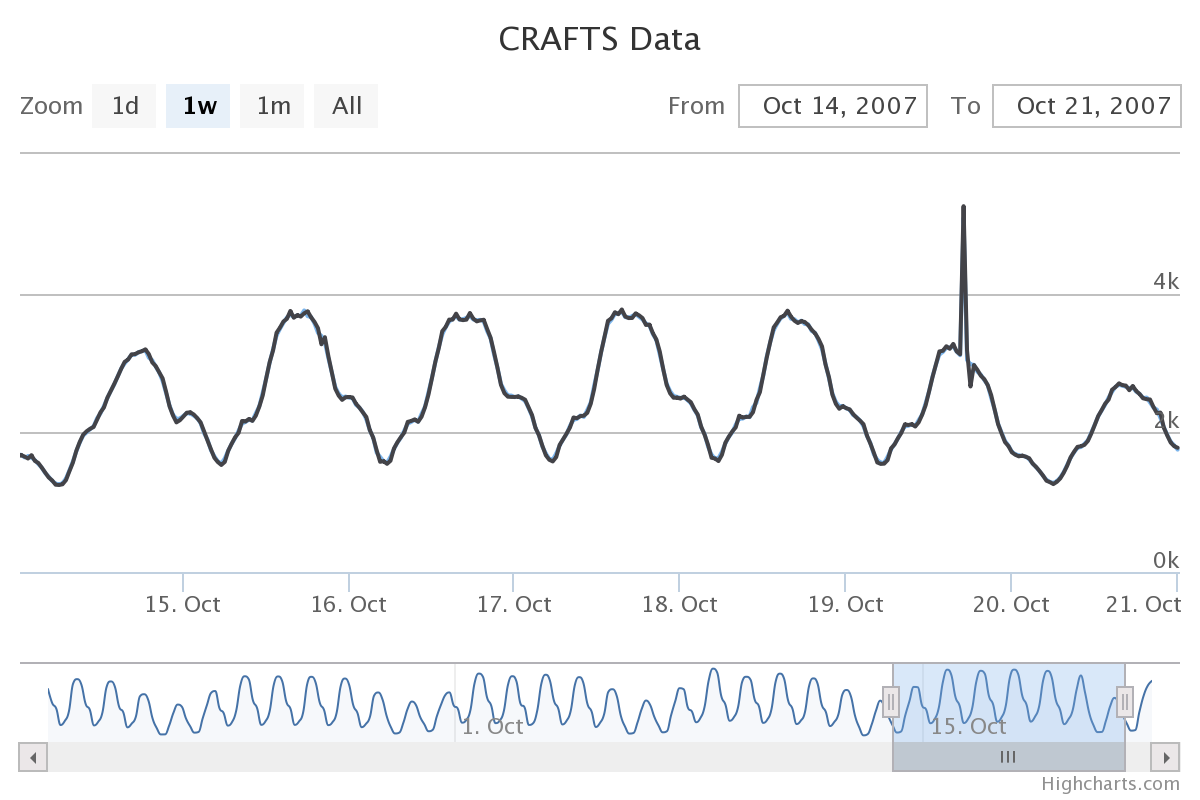
\includegraphics[width=\textwidth]{results/graphs/smoothing_horizon_spike.png}
\caption{Exponential smoothing prediction results for the horizon spike workload}
\label{fig:smoothing_hs}
\end{figure}

% Conclusions
\chapter{Conclusions}
\label{ch:conclusions}

\section{ARTS Workload Quality}
The workloads we attempted to generate through ARTS' layered transformations proved to not be as realistic as we had hoped. The transformations implemented simply could not capture all of the complexities of workloads seen in modern-day web applications. In our evaluation, even when filtering out 96\% of frequencies from the Wikipedia workload data, this still leaves over 80 dominant frequencies in the data. Representing this complexity in an ARTS workload using the current architecture would prove difficult to impossible for an average user.

\section{Predictor Evaluation}
Based on the results of our evaluation, the linear regression proved to be the most effective method of prediction. The linear regression predictor had the lowest RMSDs for regular traffic and was tolerant to every anomaly we tested.

\section{Short-term Predictors}
Both the Markov chain and exponential smoothing predictors can only make predictions a short amount of time into the future. While this gave them an advantage when predicting regular traffic, it proved to be a problem when these predictors came across anomalies. Furthermore, with a prediction horizon so small, it is impossible for the \textsf{planner} to do its job effectively. The goal of the planner is to group scaling requests together on an interval to ensure that plans are easy for an engineer to read and update in the future if necessary.

\section{Tuner Effectiveness}
In our evaluation of the FFT predictor, we found that our \textsf{tuner} implementation is not effective for all types of parameters. In the case of FFT, we saw that the \textsf{tuner} optimized parameter values were too low to filter out anomalies in the training data. There are two deficiencies in our tuning algorithm which caused this problem. First, since we weight all data equally during tuning, the effects of anomalies can become muted among the rest of the data. A solution to this would be to implement an algorithm similar to our evaluation methodology which weights error around anomalies much more heavily than regular traffic. Second, since we only observe a portion of past data in order to perform our tuning, it is possible that this window will contain no anomalies. It is also possible that the dataset contains no anomalies at all. Solving this problem would prove to be much more difficult.
\chapter{Future Work}
While we are happy with the results of our evaluation of CRAFTS and its prediction methods, there is much more work which could be done in the future to improve CRAFTS.

\section{Real-World Validation}
The best way to test CRAFTS would be to integrate it with a real running system. Not necessarily executing scaling decisions, but running predictions and making them available through the web UI.

\section{Larger Real-World Workloads}
While we attempted to contact multiple parties in order to acquire further data for evaluation, most parties were unwilling to release the sort of information we require because it could potentially be used by competitors to gain insight into revenue and other derivative metrics. In the future, it would be nice to see companies release this sort of data anonymously for the purposes of assisting the research community.

\section{Fault-Tolerance}
Since CRAFTS would form a critical part of a services infrastructure, it is important that in the event of a node-failure, another node running CRAFTS could automatically begin making predictions.

\section{Event Detection}
One of the greatest weaknesses of CRAFTS' methods is the inability to handle load events which do not occur periodically and are not anomalous. These events could include posting a breaking story on a news site or the release of a new episode in a web-series. These sorts of events need to be accounted for when scaling, but do not show the kind of periodicity which CRAFTS is designed to detect.

In the future, it would be great to see CRAFTS have the ability to detect these events and be able to recognize them in the future, or to a lesser extent, the ability for a user to be able to record an event and then initiate that event at a later time.

\section{Secondary Predictors}
Both the Markov chain and exponential smoothing predictors showed positive results making predictions a small amount of time into the future. If CRAFTS could support using one of these methods as a form of intelligent reactive scaling alongside one of its long-term prediction methods, it could improve the handling of anomalous events.

\section{Alternative Applications}
At its core, CRAFTS is a prediction pipeline. Data comes in, predictions are made, and actions are taken based on those predictions. This sort of pipeline could prove useful to other applications where these sort of automated predictions could prove useful. For example, in the field of computational finance, CRAFTS could be used to predict future stock prices and issue buy and sell orders based on its predictions.

\clearpage
\begin{flushleft}
\nocite{*}
\bibliography{bibliography}
\bibliographystyle{plain}
\end{flushleft}

\begin{appendices}
\chapter{Running CRAFTS}
\label[app]{ap:installing}
This appendix outlines instructions on how to install, setup, and run an instance of CRAFTS. Further details of how to configure CRAFTS can be found in \Cref{ap:craftsconfig}.

\section{Installation}
CRAFTS supports a number of methods of installation. Below are detailed instructions for each of the deployment methods which CRAFTS offers. This guide assumes, unless stated otherwise, that a CouchDB instance is already accessible to the user.

\paragraph{Source.}
\texttt{Git} is required in order to acquire the CRAFTS source. To download the source, simply run:

\texttt{git clone git://github.com/crafts/crafts-core.git}

\noindent
This will create the \texttt{crafts-core} folder which contains all code necessary to run CRAFTS. 

\paragraph{Pip.} Installing with pip is quick and easy. Simply run:

\texttt{pip install crafts-core}

\paragraph{Docker.} Launching a Docker container requires a copy of the source code. Inside of the \texttt{crafts-core} directory is a \texttt{Dockerfile}, build the Docker container by running the following command:

\texttt{docker build -t crafts/crafts-core .}

\noindent
The Docker container comes with a CouchDB instance pre-installed and configured.

\paragraph{Vagrant.} Launching a VM through Vagrant requires a copy of the source code. Inside of the \texttt{crafts-core} directory is a \texttt{Vagrantfile}. From within the directory, run:

\texttt{vagrant up}

\noindent
to launch the CRAFTS VM. This VM includes a local pre-configured instance of CouchDB.

\section{Setup}
Setup is as simple as using the \texttt{crafts-cli} utility to configure a running CouchDB instance. Assuming the CouchDB instance is running locally, this can be done by running:

\texttt{crafts-cli init config.json}

\noindent
Further Information about the CRAFTS configuration file can be found in \Cref{ap:craftsconfig}. If CouchDB is installed remotely, run \texttt{crafts-cli help} to see the necessary flags.

\section{Running}
The primary executable for CRAFTS is the CRAFTS daemon, \texttt{craftsd}. Each of the installation methods above, except source, will add \texttt{craftsd} to the \texttt{PATH}. If CRAFTS was installed from source, \texttt{craftsd} can be found in the \texttt{crafts} directory beneath \texttt{crafts-core}.
\chapter{CRAFTS Configuration Specification}
\label[app]{ap:craftsconfig}
CRAFTS offers a simple and extensible configuration system which exists in a JSON document stored in CouchDB. The following sections detail each of major components of CRAFTS configuration and the individual options within them.

\section{Modules}
Individual CRAFTS modules can be swapped out by changing their respective fields in the configuration file. The values for each module field should be a string which represents an importable module path. An example module configuration can be seen below.

\section{Module-Specific Configurations}
While none of the default CRAFTS modules have any additional configuration options. It is possible for extra configuration data to be passed to a custom module if necessary. To do this, create a configuration key whose name is the same as the class which the option will be passed to. Any data specified under this key will be passed directly to the module with that name.

\section{Cycles}
Most CRAFTS components are run on a configurable cycle which can be configured. Each of these cycles takes an integer value which represents the interval at which the component should be run (in seconds). The different cycles are as follows:
\begin{itemize}
\item \textbf{\texttt{monitoring\_cycle}}: The interval at which the MAL will query the monitoring data source. These requests are made in bulk so that load on the monitoring system can be kept to a minimum.
\item \textbf{\texttt{scaling\_cycle}}: The amount of time between bulk scaling requests made by the planner.
\item \textbf{\texttt{tuning\_cycle}}: How often the \textsf{tuner} should be run.
\end{itemize}

\section{Other}
The VM acquisition delay (\texttt{vm\_delay}) can also be found in the configuration, as well as the magnitude of the linear transformation applied by the \textsf{planner} (\texttt{planner\_tolerance}).

\begin{lstlisting}[language=json]
{
    "planner": "crafts.planner.simple.SimplePlanner",
    "maldriver": "crafts.mal.null.NullMAL",
    "scaler": "crafts.scaler.null.NullScaler",
    "predictor": "my.custom.package.MyPredictor",
    "tuner": "crafts.tuner.brute.BruteTuner",
    
    "MyPredictor": {"special_data": 1234},
    
    "monitoring_cycle": 86400,
    "scaling_cycle": 3600,
    "tuning_cycle": 2592000,
    
    "vm_delay": 900,
    "planner_tolerance": 1.2
}
\end{lstlisting}
\chapter{ARTS Job Configuration Specification}
\label[app]{ap:artsconfig}

ARTS jobs are configured using a JSON document as a job specification. This section outlines the different configuration options for each of the components of an ARTS job. The basic outline of a job configuration can be seen below, the individual sections will be explained in greater depth in the following sections. A complete example can be seen at the end of this appendix.

\begin{lstlisting}[language=json]
{
    "base": { ... }
    "layers": [ ... ],
    "events": [ ... ],
    "handlers": [ ... ]
}
\end{lstlisting}

\section{Base}
The ``base'' attribute specifies the initial values which the layers and events will be applied to.

\subsection{File}
Read a newline delimited file(s) of tab separated unix timestamp, value pairs.

\textbf{Arguments:}
\begin{itemize}
\item \textbf{filepath:} a unix-style glob absolute filepath to the desired input files \\
\end{itemize}

\subsection{Value}
Use a specified value as the basis of the workload.

\textbf{Arguments:}
\begin{itemize}
\item \textbf{tnot:} The initial unix time where the workload will begin
\item \textbf{duration:} The duration of the generated workload (in seconds)
\item \textbf{interval:} How often a sample should be generated (in seconds)
\item \textbf{value:} The baseline value which should be applied for the duration of the workload
\end{itemize}

\section{Layers}
Layers form the core of ARTS workloads. Layers are applied as modifiers to the base which was described in the previous section.

\subsection{Sinusoid}
Sinusoids are used to represent normal patterns seen in traffic. The resulting sine wave is centered around positive one and applied as a multiplier to the existing workload. The sinusoid transform takes an amplitude between zero and one and a frequency specified in days as parameters.

\textbf{Arguments:}
\begin{itemize}
\item \textbf{amplitude:} Amplitude of the sine wave (between 0.0 and 1.0)
\item \textbf{frequency:} The frequency of the sinusoid (in seconds)
\item \textbf{offset:} Offset in time from the start of the workload (in seconds)
\end{itemize}

\subsection{Linear}
In order to represent steady growth (or decay) seen in the real-world traffic, we offer a linear transformation. The linear transformation takes a slope as a parameter and applies that slope to each point in the workload.

\textbf{Arguments:}
\begin{itemize}
\item \textbf{slope:} Amount of slope to apply to the input data
\end{itemize}

\subsection{Blur}
Real world traffic doesn't behave like a nice straight line, there are constant minor fluctuations in traffic patterns. The blur transformation takes the current workload and adds noise based on the Gaussian distribution. Using the current data point as the mean and a configurable standard deviation, a new value is generated and inserted back into the workload.

\textbf{Arguments:}
\begin{itemize}
\item \textbf{std\_dev:} The standard deviation which should be passed to the Gaussian distribution
\end{itemize}

\section{Events}
Events are modifiers applied to the workload over a discrete time. All events take a start and end time as parameters.

\subsection{Outage}
A period of time in which all generated data is zero. The outage event takes no extra arguments.

\subsection{Spike}
A short period of time when a large multiplier is applied to the base load.

\textbf{Arguments:}
\begin{itemize}
\item \textbf{peak:} The peak multiplier to be applied to the base workload.
\end{itemize}

\section{Handlers}
Every output tuple of ARTS can be passed to one or more handlers. Handlers can be used to store the generated data or feed it directly to another application.

\subsection{FileHandler}
The file handler outputs data to the specified file in a format which it can be read in again by the file base.

\textbf{Arguments:}
\begin{itemize}
\item \textbf{filename:} Name of the output file
\end{itemize}

\subsection{CRAFTSHandler}
This handler takes the data generated by ARTS and inserts it directly into the CRAFTS intermediate store.

\textbf{Arguments:}
\begin{itemize}
\item \textbf{url:} The url of the CouchDB instance which holds the target CRAFTS database
\item \textbf{db:} The name of the CRAFTS database within CouchDB
\end{itemize}

\section{Sample Job Configuration}
\begin{lstlisting}[language=json]
{
    "base": {
        "type": "file",
        "args": {"filename": "/data/wikipedia/*"}
    }
    "layers": [
        {
            "type": "linear",
            "args": {"slope": 5}
        },
        {
            "type": "fuzzing",
            "args": {"avg": 0.1, "dev": 0.05}
        }
    ],
    "events": [
        {
            "type": "outage",
            "args": {"start": 6, "end": 10}
        },
        {
            "type": "spike",
            "args": {"start": 20, "end": 25}
        }
    ],
    "handlers": [
        {
            "type": "FileHandler",
            "args": {"filename": "new_wiki.out"}
        }
    ]
}
\end{lstlisting}
\chapter{Intermediate Storage Format}
\label[app]{ap:storage}

An example intermediate storage entry can be found at the end of this appendix. Below is a description of all fields which must be present in a valid sample document.
\begin{itemize}
\item \textbf{\_id:} Uniquely identifies the document within CouchDB. For sample documents, the id takes the form: ``\texttt\item \{role/timestamp/sample\}.''
\item \textbf{\_rev} The revision field. Used by CouchDB for consistency.
\item \textbf{timestamp:} The UTC time at which the sample was taken.
\item \textbf{role:} The role for which the sample was taken.
\item \textbf{hosts:} A list of all hosts within the role and a dictionary of the metrics recorded and their values.
\item \textbf{type:} Identifies the type of document. In this case it will always be ``sample.''
\end{itemize}

\begin{lstlisting}[language=json]
{
    "_id": "arts/2007-09-18T20:10:00/sample",
    "_rev": "1-74ec4360a516ae634edb61f840b12758",
    "timestamp": "2007-09-18T20:10:00",
    "role": "arts",
    "hosts": {
        "arts-1": {
            "requests": 3025
        }
    },
    "type": "sample"
}
\end{lstlisting}
%\chapter{CRAFTS Module Interfaces}
\label[app]{ap:craftsapi}

\section{MAL}
\begin{lstlisting}[language=python]
class MALDriver(object):
    def get_metrics(self, start, stop):
\end{lstlisting}

\section{Predictor}
\begin{lstlisting}[language=python]
class Predictor(object):
    def predict(self, window, start_time, cycle_size):
\end{lstlisting}

\section{Planner}
\begin{lstlisting}[language=python]
class Planner(object):
    
\end{lstlisting}

\section{Cluster Manager}
\begin{lstlisting}[language=python]
class Scaler(object):
    def schedule_event(self, role, time, count):

    def describe_cluster(self):
\end{lstlisting}

\section{Tuner}
\begin{lstlisting}[language=python,breaklines=true]
class ErrorMatrix(object):

def evaluate(actual_collection, predicted_collection, metric, measure):

def validate(db, role, metric, measure, start, window_size, cycle_size, num_folds, predictor_cls):

def optimization_func(params, db, role, metric, measure, start, window_size, cycle_size, num_folds, predictor_cls):

def tune(db, role, metric, measure, start, window_size, cycle_size, num_folds, predictor_cls):
\end{lstlisting}
\end{appendices}

\end{document}